\documentclass[pdftex,fontsize=12pt,a4paper,numbers=noenddot]{scrreprt}
%
%Beinhaltet alle verwendeten Pakete
% Dateiformat 
\usepackage[utf8]{inputenc}

% Sprache
\usepackage[ngerman]{babel}

% Silbentrennung
\usepackage[T1]{fontenc}  

% Serifenlose Schrift wie Arial
\usepackage[scaled]{uarial}


% Gemetrie-Packet für Seitenränder
\usepackage{geometry}

% Bilder und Grafiken
%\usepackage{graphicx}
\usepackage{pdflscape}
\usepackage{pdfpages}
\usepackage{subfigure}
\usepackage{wrapfig}




% Kopf- und Fußzeilen
\usepackage{footmisc}
\usepackage[automark]{scrpage2} 

% Aufzählungen, Tabellen, ...
\usepackage{enumitem}
\usepackage{longtable}
\usepackage{booktabs}
\usepackage{supertabular}
\usepackage{tabularx}
\usepackage{longtable}
\usepackage{colortbl}
\usepackage{multirow}

% Nummerierung von Abbildungen
\usepackage{chngcntr}

% Schriftsatz
\usepackage{textcomp}
\usepackage{float}

%Abkürzungsverzeichnis
\usepackage{acronym}

% Hyperlinks in der PDF
\usepackage{hyperref}
\usepackage{url}



\usepackage{array}

\usepackage{menukeys}
\usepackage{nameref}
\usepackage{mdframed}
%Dient zur Konfiguration von Layout und LaTeX
% Zeilenabstand
\linespread{1.15}
\setlength{\parindent}{0pt} 

%Seitenränder
\geometry{
	left=30mm,
	right=20mm,
	top=30mm,
	bottom=30mm,
}

% Befehle zur Ausgabe von Tactical Training Team
\newcommand{\TTT}{Tactical Training Team}

%Verzeichnisebenen Bilder und Tabellen
\counterwithin{figure}{section}
\counterwithin{table}{section} 

%Absand Aufzählung
\setlist[1]{itemsep=0pt}

% Farben
\usepackage{xcolor}
\definecolor{blue}{RGB}{0,0,120}
\definecolor{green}{RGB}{0,153,0}
\definecolor{backcolor}{rgb}{0.9,0.9,0.9}
\definecolor{yellow}{RGB}{255,210,0}
\definecolor{gold}{RGB}{218,165,32}
\definecolor{DarkOrchid}{RGB}{92,30,123}

%Url-Einstellungen
%\hypersetup{colorlinks=false, linkcolor=black}
\hypersetup{%
	hidelinks,
	%colorlinks=false,% hyperlinks will be black
	%linkbordercolor=black,% hyperlink borders will be black
	%pdfborderstyle={/S/U/W 1},% border style will be underline of width 1pt
	pdfauthor={\TTT}
}


% Einstellungen Kopf- und Fußzeile
\pagestyle{empty}
\clearscrheadfoot{}
\ofoot[]{\textbf{\vrule}\,\pagemark}
%\ihead[]{Tactical Training Team}
%\ohead[]{\headmark}
\chead[]{\includegraphics[width=1.05\textwidth]{./img/header}}
\addtolength{\headheight}{10mm}
\addtolength{\footskip}{-10mm}
%\setheadsepline[\textwidth]{1pt}[\color{800000}]

% Ebenen Nummerierungen
\setcounter{secnumdepth}{4} %Nummerierungsebenen
\setcounter{tocdepth}{1}   %Ebenen Inhaltsverzeichnis

%Neuer Splatentyp für Tabellen (dient dazu, dass die erste Splate zentiert werden kann)
\newcolumntype{C}[1]{>{\centering\arraybackslash}m{#1}}
%linksbündiger Spaltentyp
\newcolumntype{P}[1]{>{\raggedright\arraybackslash}p{#1}}

%Eigenen Befehl für Newline definieren
\newcommand{\nl}{\newline}

\renewcommand*{\familydefault}{\sfdefault}	
\renewcommand*\chapterheadstartvskip {%
	\vspace*{1\baselineskip plus .1\baselineskip minus .067\baselineskip}}

\begin{document}


\pagenumbering{gobble} %Seiten nicht mitzählen
%TODO: Grafisch Überarbeiten
\title{Das TTT Handbuch}
% \author{TTT Dokumentengruppe}
\begin{titlepage}
	\begin{center}
		\begin{minipage}[t]{1\textwidth}
			\centering
			\includegraphics[width=\textwidth]{./Grafiken/Abschnitt/TTTitelbild.png}
		\end{minipage}
	\end{center}
\end{titlepage}

\newpage
\pagenumbering{roman} %ab hier werden römischen Seiten als Seitenzahlen mitgezählt

\tableofcontents % Inhaltsverzeichnis

\newpage
\pagenumbering{arabic} %ab hier werden Seiten als Seitenzahlen mitgezählt
\pagestyle{scrheadings}
\renewcommand{\chapterpagestyle}{scrheadings}
\chapter*{Vorwort}
\addcontentsline{toc}{chapter}{Vorwort} 
\subsection*{Über dieses Dokument}
%\addcontentsline{toc}{subsection}{Über dieses Dokument} 
Entstanden aus dem ursprünglichen, kompakten Leitfaden zur Allgemeinen Grundausbildung im \ac{TTT} soll dieses Dokument sowohl Grünschnäbeln als auch Alten Hasen zum Erlernen und Festigen aller relevanten theoretischen Grundlagen des taktischen Spiels im \ac{TTT} dienen. 
Es ist Leitfaden, Referenzwerk und Messlatte in einem Dokument vereint. 
Wie jedes Schriftstück zur Ausbildung sollte es \textit{aktiv} gelesen werden: der Leserin oder der Leser sollte über die vermittelten Inhalte nachdenken, sie hinterfragen, diskutieren wo nötig und gewissenhaft einprägen.\\
Dieses Dokument lebt, es wird weiterentwickelt, überarbeitet, erweitert, gekürzt -- Anmerkungen, Vorschläge und Rückmeldungen konstruktiver Art werden nicht nur gewünscht, sondern gefordert. Ein hoher Standard im Spiel beginnt mit einem hohen Standard und Anspruch an alle Unterlagen, und jeder Spieler im \ac{TTT} ist nicht nur ständigen Verbesserung und Erweiterung seiner eigenen Fähigkeiten verpflichtet, sondern auch zur Verbesserung und Erweiterung des vermittelten Wissens.
Ein aufmerksamer, geübter Schütze mag den Ausgang eines Feuerkampfs für sich entscheiden -- der virtuelle Krieg wird jedoch durch Strategie, Taktik und das Wissen um das \textit{WIE} entschieden, das aus den Erfahrungen von Fehlschlägen und Triumphen herrührt. Der erste Schritt den du, lieber Leser, auf dem Weg zu einem erfolgreichen Spieler im \emph{[\ac{TTT}]} leisten musst, ist über diese Aussage zu meditieren und sie zu verstehen.\\

\textit{Train hard, play smart!}

\newpage
\subsection*{Die Grundsätze des TTT}
\label{sec:Grundsaetze}
%\addcontentsline{toc}{subsection}{Die Grundsätze des TTT} 
	\begin{itemize}
		\item Das [TTT] stellt das Training in den Mittelpunkt
		\item Das [TTT] spielt auf höchstem taktischen Niveau
		\item Das [TTT] orientiert sich in seiner Spielweise und Organisation an Kommando-Teams
		\item Das [TTT] pflegt und lebt das Battle Buddy System
		\item Das [TTT] lässt im Spiel keinen Kamerad zurück, jedem Notruf wird Folge geleistet
		\item Das [TTT] ist eine offene Community -- jeder kann am Training oder den Events grundsätzlich teilnehmen
		\item Die [TTT] Community wird geführt wie ein aktives, ergebnisorientiertes Unternehmen -- die Stammspieler sind das wichtigste Kapital	
	\end{itemize}

\vspace*{\fill}
	\begin{figure}[htbp]
		
\includegraphics{./img/by-nc-sa}
	\end{figure}

Some pictures and graphics of this document was created using ARMA 3.\\
ARMA 3 is a registered trademark of Bohemia Interactive a.s.\\
See www.bistudio.com for more information.

\part*{ATCHUNG hierbei handelt es sich um eine BETA-Version, dementsprechend können Abweichungen zu Training und Ensteigerevent existieren}
\part{Truppenordnung \& Basisentnisse}
%Truppengattungen
\chapter{Truppenordnung}
In diesem Abschnitt werden die einzelnen Strukturelemente und die Organisation des \ac{TTT} während einer typischen Mission erklärt.\\
Die hier vorgestellten Strukturen basieren dabei auf der im Laufe der Zeit gesammelten Erfahrung, was in ArmA funktioniert und was nicht und sind verpflichtende Vorgabe für jeden Missionsbauer. Ausnahmen von diesen Strukturen müssen vorher angefragt und genehmigt werden.\\
Da im \ac{TTT} sowohl deutsche als auch amerikanische Strukturen benutzt werden, werden die amerikanischen Namen jeweils in Klammern zusätzlich zu den deutschen Namen genannt.

\section{\acf{OPL} / \acf{HQ}}
\begin{wrapfigure}{r}{0.35\textwidth}
	%\vspace{-15pt}
	\centering 
	\includegraphics[width=0.3\textwidth]{../img/truppenordnung/opl/opl}
	%\caption{Beispiel einer \ac{OPL}}
	%\vspace{-30pt}
\end{wrapfigure}	

Die \ac{OPL} ist die höchste Instanz innerhalb einer Mission. Sie hat den Oberbefehl über alle Einheiten inne, koordiniert das allgemeine Vorgehen innerhalb der Mission und verwaltet die Zuordnung der unterstützenden Einheiten zu den kämpfenden Einheiten. Sie kommuniziert grundsätzlich nur über die Long-Range mit ihren untergeordneten Einheiten.
\par\bigskip
Die \ac{OPL} ist folgendermaßen aufgebaut:
\begin{itemize}
	\item Operationsleiter\,/\,\acs{OPL} (\acf{CO}): Der Oberbefehlshaber der Mission. Er gibt die Befehle und erstellt "den großen Plan".
	\item stellv. \ac{OPL} (\acf{XO}): Unterstützt den \ac{OPL} bei seinen Aufgaben, typischerweise beim Funken mit den untergeordneten Trupps. Kann jedoch auch alle weiteren Aufgaben übernehmen, die ihm der \ac{OPL} überträgt -- er ist Mädchen für alles. Bewährt hat sich das Prinzip, dass der \ac{OPL} den eingehenden Funk übernimmt (Anfragen von anderen Trupps) und der stellv. \ac{OPL} den ausgehenden Funk (Abfragen von Statusberichten, Übermittlung von neuen Befehlen).
\end{itemize}
Ergänzt werden kann die \ac{OPL} durch maximal 4 Spieler, welche folgende Rollen einnehmen können:
\begin{itemize}
	\item Funker (\acf{RO}): ein zusätzlicher Funker, um die \ac{OPL} zu unterstützen, kann auf eine Spezialrolle beschränkt sein und für diese eine eigene LR-Frequenz bekommen (so kann es z.\,B. bei einer Mission mit vielen Lufteinheiten sinnvoll sein, jemanden zu haben, der sich auf einer eigenen Frequenz nur um die Koordination der Lufteinheiten um das Flugfeld kümmert und zentraler Ansprechpartner aller Lufteinheiten für Start-\,/\,Landemanöver ist)
	\item Aufklärungsoffizier (\acf{IO}): Sammelt alle verfügbaren, relevanten Daten und leitet diese gegebenenfalls an andere Trupps weiter. Hat meistens eine eigene, "große" Drohne (Greyhawk\,/\,Global Hawk) zur Feindaufklärung.
	\item freie Rolle (maximal einmal): je nach Mission kann es sinnvoll sein, dem \ac{OPL} einen Sanitäter, einen Nahsicherer, einen Fahrer o.\,Ä. zur Seite zu stellen
\end{itemize}
Je nach Größe und Struktur der Mission kann die \ac{OPL} identisch sein mit
\begin{itemize}
	\item der Sektionsführung, falls die Truppstruktur der Mission nur aus einer Sektion besteht
	\item der Zugführung, falls die Truppstruktur der Mission nur aus einem Zug besteht (egal ob Infanteriezug, Panzerzug oder mechanisierte Infanterie). Dies ist die einzige Ausnahme, in der die \ac{OPL} per Short-Range statt Long-Range mit ihren untergeordneten Einheiten kommuniziert.
\end{itemize}
Die OPL hält typischerweise einen sehr großen Abstand zu ihren Truppen - oft bleibt sie auch durchgehend in der Basis.

\section{Sektionsführung / Platoon Lead (PLT)}
\begin{wrapfigure}{r}{0.4\textwidth}
	\vspace{-25pt}
	\centering 
	\includegraphics[width=0.3\textwidth]{./img/truppenordnung/sektionsfuehrung/sektionsfuehrung}
	%\caption{Beispiel einer Sektionsführung}
	\vspace{-90pt}
\end{wrapfigure}	
Die Sektionsführung ist ein Bindeglied zwischen OPL und Zugführung, um die OPL zu entlasten. Einer Sektionsführung sind mindestens zwei, maximal vier Züge unterstellt. Ab drei Zügen in einer Mission ist die Sektionsführung zwingend erforderlich, darunter optional.\\

Die Sektionsführung ist folgendermaßen aufgebaut:
\begin{itemize}
	\item Sektionsführer\,/\,Platoon Lead (PLT): Er leitet die ihm untergeordneten Züge. Kommuniziert wird über Long-Range - entweder über die individuellen Frequenzen der einzelnen Züge oder über die Task-Force-Frequenz (siehe nächstes Kapitel).
	\item Funker / Radio Operator (RO): Übernimmt die Kommunikation zur OPL und anderen Einheiten.
\end{itemize}
Ergänzt werden kann die Sektionsführung bei Bedarf durch:
\begin{itemize}
	\setlength\itemsep{0em}
	\item einen Gefechtssanitäter\,/\,Combat Medic (CM) zur Versorgung im Feld.
	\item einen Fahrzeugführer\,/\,Nahsicherer zur selbstständigen Verlegung
\end{itemize} 
Die Sektionsführung befindet sich typischerweise etwas weiter entfernt hinter den ihr unterstellten Zügen.

\input{./truppenordnung/zugfuehrung}
\section{Infanterietrupp / Fireteam (FT)}
\begin{wrapfigure}{R}{0.35\textwidth}
	\vspace{-50pt}
	\centering 
	\includegraphics[width=0.2\textwidth]{../img/truppenordnung/infanterie/infanterie}
	%\caption{Beispiel eines Infantrietrupps}
	\vspace{-90pt}
\end{wrapfigure}
Die Infanterie bildet den Kernbestandteil vieler Missionen. Ein Infanterietrupp ist immer Teil eines Zuges und besteht aus 4 oder 6 Mann. Mögliche Positionen innerhalb eines Infanterietrupps sind:
\vspace{3.5cm}
\begin{longtable}{@{}P{0.4\textwidth}P{0.4\textwidth}@{}}
	\toprule
	Deutsche Bezeichnung & Englische Bezeichnung\\
	\midrule
	Truppführer (TF) & Fireteam Leader (FTL)\\
	Grenadier (GRE) & \\
	Leichter MG-Schütze (LMG) & Automatic Rifleman (AR)\\
	Mittlerer MG-Schütze & Medium Machine Gunner (MMG) \\
	MG-Assistent & Assistant Machine Gunner (AMG)\footnote{notwendig für MMG}\\ 
	Leichter Panzerabwehrschütze & Light Anti Tank (LAT)\\
	Schwerer Panzerabwehrschütze & Heavy Anti Tank (HAT)\\
	Panzerabwehr-Assistent & Assistant Anti Tank (AAT)\footnote{notwendig für HAT}\\ 
	Luftabwehrschütze & Anti-Air (AA)\\
	Pionier & Pioneer (PIO)\\
	Gefechtssanitäter & Combat Medic (CM)\\
	Schütze & Rifleman (RI)\\			
	\bottomrule					
\end{longtable}


Auf eine sinnvolle Einteilung in Buddy"=Teams (z.\,B. bei Positionen, die einen Assistenten erfordern), ist hierbei zu achten.\\
Die Kommunikation erfolgt ausschließlich über Short-Range, der Truppführer schaltet sich über seine Additional-Short-Range auf den Zugkanal auf, um sich mit der Zugführung und den anderen Truppführern im Zug abzusprechen. Die Nummer 2 im Trupp kann sich ebenfalls auf den Zugfunk aufschalten, jedoch nur mithören und nicht funken -- es sei denn, der Truppführer fällt aus und die Nummer 2 übernimmt.

\section{Spezialtrupp}
\includegraphics[width=20mm]{./img/truppenordnung/spezialeinheiten/sf1}\quad
\includegraphics[width=20mm]{./img/truppenordnung/spezialeinheiten/sf2}\\
Spezialtruppen sind infanteristische Einheiten bestehend aus zwei bis sechs Mann mit einem klaren Aufgabenschwerpunkt -- dies kann vom klassischen Zwei"=Mann"=Scharfschützenteam bis zum Sechs-Mann-Kampftauchertrupp gehen. Sie sind die flexibelsten Einheiten innerhalb des TTTs und können entweder autark arbeiten oder im Verbund mit einem anderen Trupp oder Zug. Pro Mission existieren maximal zwei autark operierende Spezialtruppen, im Verbund mit einem Zug maximal einer.\\
Kommunikation erfolgt über Long"=Range, beim Arbeiten im Verbund zusätzlich über die Additional"=Short"=Range (Zugfunk). Kämpfende Einheiten wie z.B. Kommandotrupps oder Kampftaucher, in denen der Truppführer viel Mikromanagement leisten und der Trupp in direkte Feuergefechte verwickelt wird, benötigen zwingend einen separaten Funker. In unterstützenden Einheiten wie z.B. Aufklärungsteams oder Mörserteams, die voraussichtlich nicht in direkte Feuergefechte verwickelt werden, kann (muss aber nicht) der Truppführer die Long"=Range"=Kommunikation mit übernehmen.\\
Mögliche Aufgabenschwerpunkte eines Spezialtrupps sind z.B.:

\begin{itemize}
	\setlength\itemsep{0em}
	\item JTAC-Team
	\item Aufklärungsteam (UAV)
	\item Autonome Kampfeinheit (UGV)
	\item Mörserteam
	\item schwere Feuerunterstützung (Schweres Maschinengewehr (HMG) / Granatmaschinengewehr (GMG))
	\item (schwere) Panzerabwehr / Flugabwehr (falls nicht bereits im Zug vorhanden)
	\item Pionier-Team (falls nicht bereits im Zug vorhanden)
	\item medizinische Versorgung/Unterstützung (falls kein MedEvac in der Mission vorhanden)
	\item Kommandokräfte (Infiltration)
	\item Scharfschützenteam
	\item Kampftaucher
\end{itemize}
Bei entsprechenden Rollen (schwere Waffen, Mörser, etc.) ist auf das Vorhandensein eines entsprechenden Assistenten zu achten.
\section{Logistik}
\includegraphics[width=20mm]{../img/truppenordnung/logistikMedevac/silber}\linebreak
Silber -- Bussard -- Stellt Fahrzeuge und Personal bereit, mit denen Transport und Logistik durchgeführt werden.
\section{MedEvac}
\includegraphics[width=20mm]{../img/truppenordnung/logistikMedevac/weiss}\\
Weiß -- \acf{MedEvac} -- Unterstützt Operationen mit Versorgungs- und Transportkapazität für Verwundete.
\section{Close Air Support}
\includegraphics[width=20mm]{../img/truppenordnung/logistikMedevac/silber}\\
Silber -- Adler -- Stellt Fahrzeuge und Personal bereit,  Gefechtsunterstützung (\ac{CAS}) und Geleitschutz durchgeführt werden.
\input{./truppenordnung/mechanisierte_infanterie}
\input{./truppenordnung/kampfpanzer}
\input{./truppenordnung/artillerie}

% Grundlagen
\chapter{Basiskenntnisse}
%TODO Kurze Beschreibung

\input{./basic/formation/formation}
\pagebreak

\section{Sicherungsbereiche}
Die Sicherung wird in Bewegung immer über die Uhrzeit ausgegeben. Sowohl in Fahrzeugen als auch zu Fuß in Marschformationen. Die Marschrichtung ist immer 12 Uhr.

\subsection{Rundumsicherung}
\label{subsec:360sicherung}
Rundumsicherung bedeutet, dass 360° vom Trupp abgesichert werden. Jeder Soldat hat dazu den Auftrag, ein Viertel des \glqq Kreises\grqq\space abzusichern. Eine Rundumsicherung kann aus dem Marsch oder in einer Stellung vollzogen werden. In einer Stellung geht es nicht darum, einen perfekten Kreis zu bilden -- sondern sich in Deckung zu bewegen und von dort aus seinen Sektor zu sichern. Je nach Bedarf kann der Truppführer sich, um z.\,B. zu funken, eine 4 Mann Sicherung aufbauen lassen.
\begin{table}[h]	
	\caption{Sicherungsbereiche der Rundumsicherung für Soldaten}
	\vspace{2.5mm}
	\label{tab:360er}
	\centering
	\begin{tabular}{lll}
		\toprule
		Nr. & Sicherungsrichtung 4 Mann & Sicherungsrichtung 6 Mann\\
		\midrule
		1 & 12 Uhr 	& 12 Uhr\\
		2 & 9 Uhr	& 12 Uhr\\
		3 & 3 Uhr	& 3 Uhr\\
		4 & 6 Uhr	& 6 Uhr\\
		5 &			& 9 Uhr\\
		6 &			& 6 Uhr\\
		\bottomrule
	 \end{tabular}
\end{table}
		
\begin{figure}[h]
	\centering
	\subfigure[4-Mann 360er]{\includegraphics[width=0.49\linewidth]{../img/basic/sicherung/360grad_sicherung_4mann}}
	\subfigure[6-Mann 360er]{\includegraphics[width=0.49\linewidth]{../img/basic/sicherung/360grad_sicherung_6mann}}
	\label{fig:360er}
\end{figure}

\subsection{180°"=Sicherung}
	Die 180-Grad-Sicherung ist eine Halbkreis-Sicherung. Sie wird in der Regel an Mauern angewandt oder in einer Stellung, um ein zu beobachtendes Gelände abzusichern, wenn der Rückraum als absolut sicher gilt. Zu beachten ist, dass die 180° Sicherung nicht unmittelbar an der Mauer sondern etwa 1m entfernt aufgebaut wird. So können einzelne Soldaten oder Trupps hinter der Sicherung kreuzen, ohne in den eigenen Feuerbereich treten zu müssen.\linebreak
	\begin{figure}[htbp]
		\centering
		\includegraphics[width=0.8\linewidth]{../img/basic/sicherung/180grad_sicherung_4mann}
		\caption{180° Sicherung an Mauer 4 Mann}
	\end{figure}
		
		\begin{figure}[htbp]
			\centering
			\includegraphics[width=0.8\linewidth]{../img/basic/sicherung/180grad_sicherung_6mann}
			\caption{180° Sicherung an Mauer 6 Mann}
		\end{figure}
\newpage
\section{Das Buddy-System}
	Das Buddy"=System ist ein grundlegender Bestandteil des \textbf{TTT}s (\ref{sec:Grundsaetze}). Dabei ist das Buddy"=Team die kleinste organisatorische Einheit, das solide Fundament jedes Trupps und die Lebensversicherung jedes Soldaten. Damit dieses System funktioniert ist es erforderlich, dass die Buddy"=Mitglieder aufeinander aufpassen, an einem Strang ziehen und sich gegenseitig unterstützen. Weiterhin können Buddy"=Teams als eine Einheit agieren, die spezielle Aufgaben übernehmen. Beispiele hierfür wären Schwerpunktwaffen, Fahrzeugbekämpfung, Aufklärung oder Führung, um nur einige Möglichkeiten zu nennen. Gegenüber den genannten Vorteilen existieren auch Nachteile, die nicht ungenannt bleiben sollen. Ein leicht erkenntlicher Nachteil ist, dass ein Buddy"=System aus Menschen besteht, die zusammenarbeiten müssen. Bis dieses Team optimal zusammenwirkt, kann unterschiedlich viel Zeit vergehen. Dies kann jedoch unter regelmäßiges anwenden beschleunigt werden. Weiterhin können die Spezialisierung von Buddy"=Teams in gewissen Situationen von Nachteil sein. Dies kann jedoch durch den Truppführer kompensiert werden. Damit das Buddy"=System alle Qualitäten hervorbringt sollte jeder Spieler, sowohl Stammspieler, als auch Gast, danach streben ein besserer Buddy zu werden.
	
	Während der Mission sollte sich ein Spieler über folgenden Dinge seines Buddys im Klaren sein:
	\begin{itemize}
		\item Position
		\item Zustand 
		\item Ausrüstung und momentaner Munitionsstand
		\item Grobe Blickrichtung oder Sicherungsrichtung
	\end{itemize}
	Diese Informationen sollten durch die Kommunikation mit seinen Buddy aktuelle gehalten werden (kleine Kampfgespräch). Beispiele hierfür sind z.\,B. die Beobachtungsrichtung, Feindbekämpfung, Positionswechsel oder Richtungsänderungen. Im  \ac{CQB} erfolgt die Kommunikation in anderer Form (siehe \ref{CQB}).
	Nicht zu vergessen ist, dass Eigensicherung vor Fremdsicherung geht. Das heißt, der Buddy wird erst dann gerettet, wenn sichergestellt ist, dass die Rettung erfolgreich verläuft. Denn ein verletzter Buddy kann seinen Buddy nicht effektiv helfen.
\section{Funken und Kommunikation}
	Zum generellen Gebrauch des Funkgeräts sei auf den TFAR-Mod verwiesen. Weiterhin sollte die eigene Stimmlautstärke nicht auf >>Laut<<, (>>yelling<<) stellen. Dies verhindert, dass die Kommunikation, mehreren eng geführten Trupps, vermischt wird.\\
	Grundsätzlich sollten alle wichtigen Meldungen dem Truppführer, über die Trupp interne Funkfrequenz, mitgeteilt werden.
 
\subsection{Kontakmeldungen}
	Kontaktmeldungen sollten im Optimalfall nach einem bestimmten Schema ablaufen. Hierbei gilt im Gefecht wird nicht jede Kontaktmeldung perfekt sein. Dennoch sollte die Meldung möglichst nach diesen Schema erfolgen.
	\begin{itemize}
		\setlength{\itemsep}{-4pt}
		\itemsep-4pt
		\item >>Kontakt<< oder >>Freunde<<
		\item Anzahl 
		\item Was
		\item Wo (Grobe Richtung, Landmarke (ggf. verfeinern), Gradzahl auf Kompass) 
		\item Entfernung
		\item Weitere Angaben (Bewaffnung, Alarmzustand (heiß oder kalt), Bewegungsrichtung, ...)
	\end{itemize}

	Beispiele:
	\begin{longtable}{P{0.95\linewidth}}
	\toprule
	Kontakt -- 1 feindlicher \acs{SPZ} -- auf 4 Uhr -- Rechts über der Hütte -- auf 95° -- ca. 500m\\
	\rcg Kontakt -- 3 Infanteristen -- auf 1 Uhr -- Kommen über den Hügel -- bei 25° -- ein \acs{MG} -- ca. 300m -- kalt\\
	\bottomrule
	\end{longtable}	
\subsection{Funkgespräch unterbrechen}
	In bestimmten Situationen ist es erforderlich eine aktuelle Funkmeldung oder ein Gespräch zu unterbrechen, um eine Meldung abzusetzen von höherer Priorität, wie z.\,B. Feindkontakt zu melden. Dabei stellt >>Break, Break<< eine kurze und prägnante Aussage dar.\\
	Beispiel:
	\begin{longtable}{P{0.95\linewidth}}
	\toprule
	TF: >>Wir gehen folgendermaßen vor Bud\dots<<\\
	\rcg TM: >>Break, Break<< \dots >>Kontakt feindlicher Trupp auf 2 Uhr 100\,m nähert sich<<\\
	TF: >>Verstanden, Feuer frei!<<\\
	\bottomrule
	\end{longtable}		

\subsection{Sonstige Meldungen}
	\paragraph*{Betreten von Fahrzeugen}
	\label{para:fahrzeug-betreten}
	Bei betreten oder verlassen von Fahrzeugen wird kurz und prägnant gemeldet, dass der Soldat das entsprechend Betreten betreten oder verlassen hat. Damit erhält der TF die Information wo sein Trupp sich befindet und die Truppmitglieder wissen wie sie sich zu verhalten haben. (Erst wenn 3 meldet, dass er sitzt kann 2 aufsitzen)\\
	Beispiel: >>3, Sitzt<<

	\paragraph*{Sicherungsposition melden}
	Meldungen über aufgebaute Sicherung sind nützlich Details, die den TF über den Status der Sicherung informieren. \\
	Beispiel: >>Hier 6, Sicherung nach 6 Uhr steht<<

	\paragraph*{Trupp in Bewegung}
	Das letzte Truppmitglied (üblw. die Nr.\,6) meldet den Status der Bewegung.\par
	Beispiel:
	\begin{longtable}{P{0.95\linewidth}}
	\toprule
	TF: >>Trupp Marsch<<\\
	\rcg TM 6: >>Trupp in Bewegung<<\\
	\bottomrule
	\end{longtable}		
	
	\paragraph*{Statusmeldung und durchzählen}
	\label{sec:Status}
	Nach heftigen, ggf. unübersichtlichen Feindbeschuss ist es sinnvoll den Status des Trupps abzufragen. Die Meldung gibt den Gesundheitsstatus und Munitionsstatus, mittels Ampelsystem durch. Sollte der Truppführer nicht erreichbar sein kann auch ein Trupp Mitglied die Statusabfrage anordnen.\par
	Es wird generell von 1 an heruntergezählt. (Wenn 1 die Statusmeldung anordnet entfällt die Meldung der 1 i.\,d.\,R.)  \\
	Aufbau der Meldung: >>Nummer, Gesundheitsstatus, ggf. Besonderheiten<<
	\par\medskip
	Beispiel:
	\begin{longtable}{P{0.95\linewidth}}
	\toprule
	>>1 hier 5, Kommen<< \dots (keine Reaktion)\\  
	>>Hier 5, Trupp Status durchgeben<< \dots (kurz warten 1 und 2 melden sich nicht)\\ 
	\rcg >>Hier 3, Status Rot, Gelb<< \dots\\ 
	\rcgg >>Hier 4, Status Grün, Grün, zwei Verletzte auf dem Hügel<< \dots usw.\\
	\bottomrule
	\end{longtable}		

\subsection{Wichtigste Funkabkürzungen und Begriffe}
	\begin{longtable}{p{0.1\linewidth}p{0.25\linewidth}p{0.05\linewidth}p{0.1\linewidth}p{0.35\linewidth}} 
		\toprule
		\acs{SPZ}	& \acl{SPZ}	&& Standby	& Bitte warten \hfil\\ 
		\midrule
		\acs{KPZ}	& \acl{KPZ}	&& Kalt		& keine Gegner; Gegner haben uns nicht erkannt\\ 
		\acs{AA}	& \acl{AA}	&& Heiß 		& Gegner eröffnen Feuer, haben uns entdeckt \\ 
		\acs{AT}	& \acl{AT}	&& \acs{OPL}	& \acl{OPL} \\ 
		\acs{MG}	& \acl{MG}	&& \acs{CAS}	& \acl{CAS} \\ 
		\bottomrule
	\end{longtable}



\subsection{Kommandos -- die wichtigsten Befehle}
\label{sec:kommando}
\medskip %TODO Kurzer Satz
\paragraph*{Kommando: >>Deckung!<<}
	Die Deckung ist ein situationsbedingter Aufenthaltsort.	\par
	Wird man vom Feind überrascht, ist der Soldat angewiesen, sofort Deckung im nahen Umfeld (Radius 20 Meter) zu suchen – ohne die Trupp-Struktur aufzulösen. Dabei gilt zu beachten, dass die Buddy-Teams immer im Verbund bleiben.\par
	Als Deckung zählt alles, was als beschusssicher gilt: Häuser, Felsen, Mauern, Senken. Ist keine Deckung in Laufweite, wird sofort Bodenlage eingenommen und auf den Feind ausgerichtet. Bei indirektem Beschuss (Granaten, etc.) wird ein besonders weiter Abstand zwischen den Kameraden gesucht.
	\par\medskip
	Der Befehl vom Truppführer lautet >>Deckung!<< oder als ausführlicheres Beispiel >>Deckung, 6 Uhr, hinter der Mauer!<<

\paragraph*{Kommando: <<Bezieht Stellung bei \dots!>>}
	Die Stellung ist ein selbst gewählter Aufenthaltsort.\par
	Die Stellung ist idealerweise ein gewählter und geschützter Aufenthaltsort (Haus, Senke, Felsen, Mauer) und lässt sich leicht verteidigen. Die Soldaten haben dabei maximale Deckung eingenommen und sichern.\par
	Der Truppführer gibt den Befehl aus, um einen Aufenthaltsort festzulegen, wo sich der Trupp aufhalten soll. Daraus folgt automatisch, dass der Trupp den Ort erreicht und vorläufig sichert. Der Sicherungsschwerpunkt liegt automatisch auf vermutete Feindstellungen. Mit dem Zusatz <<gedeckt>> betont er, dass der Trupp eine Aufklärung durch den Feind unter allen Umständen vermeiden soll. In der Praxis: Nähern in die gedeckte Stellung unter Sicht- und Deckungsschutz. Dort in die Stellung getarnt beziehen und halten. In der Stellung erfolgt vom Truppführer:

\paragraph*{Kommando: >>Bekämpfen \dots!<<}
	Der Soldat soll einen erkannten Feind bekämpfen. Hierbei ist es wichtig, genau abzuwägen, wie viel Einweisung benötigt wird, damit das Kommando erfolgreich ausgeführt werden kann. Der Soldat meldet bei erfolgreicher Absolvierung des Auftrags >>Gegner, YXZ, bekämpft!<<

\paragraph*{Kommando: >>Feuer frei!<<}
	Das ist die direkte Anweisung, JETZT zu schießen. Kann ergänzt werden mit >>Feuern, 3 Salven<< oder sonstigen Einschränkungen.

\paragraph*{Kommando: >>Unterdrückungsfeuer!<<}
	Das ist die direkte Anweisung, in die generelle Richtung des Gegners zu schießen, um ihn in die Deckung zu zwingen und ihn an Gegenfeuer oder Manövern zu hindern.

\paragraph*{Kommando >>Gezieltes Feuer!<<}
	Das ist die direkte Anweisung, den Gegner mit gezielten Salven oder Einzelschüssen direkt zu treffen -- also das Gegenteil vom Unterdrückungsfeuer. In der Regel wird bei der Feuerfreigabe erwartet, dass gezieltes Feuer abgegeben wird.

\paragraph*{Kommando >>Feuerfreigabe erteilt<<}
	Grundsätzliche Freigabe den Feuerkampf eigenständig zu eröffnen. Das heißt, sobald Gegner in Sicht sind und der Feuerkampf ist aussichtsreich, darf geschossen werden. Dies gilt bis zum Widerruf.

\paragraph*{Kommando >>Feuer nur auf Freigabe<<}
	Vor dem Schuss muss Feuerfreigabe angefordert werden.

\paragraph*{Kommando: >>Stopfen!<<}
	Der Soldat stellt sofort das >>Schießen<< ein.

\paragraph*{Kommando: >>Bezieht Stellung bei \dots!<<}
	Die Stellung ist ein selbst gewählter Aufenthaltsort. Idealerweise ist diese ein geschützter Aufenthaltsort (Haus, Senke, Felsen, Mauer) und lässt sich leicht verteidigen. Die Soldaten haben dabei maximale Deckung eingenommen und sichern.\par
	Der Truppführer gibt den Befehl aus, um einen Aufenthaltsort festzulegen, wo sich der Trupp aufhalten soll. Daraus folgt automatisch, dass der Trupp den Ort erreicht und vorläufig sichert. Der Sicherungsschwerpunkt liegt automatisch auf vermutete Feindstellungen. Mit dem Zusatz >>gedeckt<< betont er, dass der Trupp eine Aufklärung durch den Feind unter allen Umständen vermeiden soll. In der Praxis: Nähern in die gedeckte Stellung unter Sicht- und Deckungsschutz. Dort in die Stellung getarnt beziehen und halten. In der Stellung erfolgt vom Truppführer:
		\begin{itemize}
			\item Kontaktaufnahme mit dem Zugführer 
			\item Geländetaufe 
			\item Verteilung von Feuerbereichen 
			\item Vorausschauende Planung (Wegplanung, Korridore, weitere Stellungen) 
			\item Kommando: <<Bezieht gedeckte Stellung bei \dots!>> 
		\end{itemize}

\paragraph*{Kommando: >>Wechselt die Stellung!<<}
	Der taktische Stellungswechsel ist ein eigenständiger Positionswechsel in eine andere Stellung -- beispielsweise, weil man befürchtet, die Stellung ist vom Feind bereits aufgeklärt wurde und damit Feindfeuer erwartet. Das gilt besonders nach Feuerüberfällen -- häufige Stellungswechsel sind sehr effektiv um Gegner zu verwirren.

\paragraph*{Kommando: >>Nehmt ein!<<}
	Das bedeutet für den Trupp, dass eine gegnerische Stellung und\,/\,oder ein Gebiet (umkämpft oder nicht umkämpft) unter allen Umständen eingenommen und erobert werden soll. Einnehmen signalisiert dem Soldaten, dass Feindkontakt möglich ist.

\paragraph*{Kommando: >>Haltet \dots!<<}
	Das bedeutet nichts anderes als IN der Stellung zu verbleiben und diese zu verteidigen.

\paragraph*{Kommando: >>Melden bei Vollzug!<<}
	Der Soldat soll, sobald er seinen Auftrag erledigt hat, sich beim Auftraggeber melden. Dies kann per Funk oder direkter Ansprache erfolgen.

\paragraph*{Kommando: >>Status<<}
	Der Soldat gibt den Gesundheitsstatus und seinen Munitionsstatus durch. Dieses Kommando deckt sich mit den Abschnitt \ref{sec:Status}.

\subsubsection{Feuerfreigaben}
	Es versteht sich von selbst, dass wir nicht auf alles zur jeder Zeit schießen können. Daher gibt es die sogenannten Feuerfreigaben, wann geschossen werden darf und wann nicht. Wir unterschieden 3 Typen:

\paragraph*{>>Feuerstatus rot<<}
	Alternativ: >>Status -- Feuer halten<<\par
	Nur schießen, wenn es um das blanke Überleben geht. >>Feuer halten<< wird ausgegeben, wenn wir leise und unerkannt in eine Stellung einsickern wollen. Feuergefechte sollten unter allen Umständen vermieden werden, da Schüsse die eigene Position verraten und Kameraden gefährden können.
\paragraph*{>>Feuerstatus gelb<<}
	Alternativ: >>Status -- Feuer erwidern<<\par
	Bei erkanntem Feind, der uns noch nicht uns bekämpft (kalt), wird der Feind gemeldet und es wird gewartet, was der Truppführer entscheidet. Es darf bei Beschuss auf die eigene Stellung zurückgeschossen werden, wenn der Feind klar erkannt wurde (heiß).
\paragraph*{>>Feuerstatus grün<<}
	Alternativ: >>Status -- Feuer frei<<\par
	Jeder erkannte Feind darf bekämpft werden. Diese Freigabe wird beispielsweise bei einem Feuerüberfall gegeben, oder in einem Verteidigungsszenario aus einer befestigten Stellung heraus.
%
\subsubsection{Zusammenfassung Kommandos}
	\begin{longtable}{p{0.3\linewidth}p{0.65\linewidth}} 
		\toprule
		\textbf{Befehl} & \textbf{Bedeutung}\\
		\midrule
		Deckung! & Beschusssichere Stellung in 20\,m Umkreis suchen mit Buddy, ansonsten auf den Boden legen.\\
		Bekämpfen! & Erkannten Feind bekämpfen, bei Vollzug mit >>Bekämpft<<, bestätigen.\\
		Feuer Frei! & Feuer sofort eröffnen.\\
		Unterdrückungsfeuer! & Durch gezielte Schüsse in Feindrichtung diesen am kämpfen oder bewegen hindern.\\
		Gezieltes Feuer! & Gegner mit gezielten Salven oder Einzelschüssen bekämpfen. Wird bei \glqq Feuer frei\grqq\, vorausgesetzt.\\
		Feuerfreigabe erteilt! & Ist Feuerkampf aussichtsreich, darf dieser begonnen werden.\\
		Feuer nur auf Freigabe! & Feuerkampf ist nur auf expliziten Befehl hin zu beginnen.\\
		Stopfen! & Das Feuern ist \textbf{sofort} einzustellen.\\
		Bezieht Stellung bei \dots! & Mit Trupp oder Buddy zu einer Position gehen und entsprechende Sicherung aufbauen.\\
		Wechselt die Stellung! & Mit Trupp oder Buddy oder alleine in andere Stellung verlegen.\\
		Nehmt \dots ein! & Das angegebene Ziel ist unter allen Umständen zu erobern und zu sichern.\\
		Haltet! & In der Stellung bleiben und diese verteidigen.\\
		Melden bei Vollzug! & Rückmeldung bei Abschluss eines Befehls oder Auftrags.\\
		Status! & Gesundheitsstatus und Munitionsstatus mit Ampelsystem durchgeben.\\
		\bottomrule
	\end{longtable}

\input{./basic/gelaende-bewegung/gelaende-bewegung}
\pagebreak
\section{Umgang mit Fahrzeugen}
\subsection{Auf- und Absitzten}
Fahrzeuge (sowohl Boden-, als auch Luftfahrezeuge) werden in umgekehrte Trupp Reihenfolge betreten. (Siehe auch \nameref{para:fahrzeug-betreten})
\par\medskip
\begin{hint}
	Kommando >>Verlassen<<: Alle Truppteile verlassen das Fahrzeug
\end{hint}
\begin{hint}
	Kommando >>Absitzen<<: Schütze bleibt, Fahrer bleibt im Fahrzeug bzw. in der Nähe des Fahrzeuges, restliche Personen verlassen das Fahrzeug und bauen Sicherung auf.
\end{hint}

\subsection{Sicherungsbereich}
Der Sicherungsbereich nach Verlassen des Fahrzeuges entspricht den Standsicherungsbereichen für  Trupps (siehe \nameref{subsec:360sicherung}, \autoref{subsec:360sicherung}). Mehrere Trupps können sich z.\,B. 180° Sicherungsbereiche abstimmen. 
\par\medskip
Wichtig:
\begin{itemize}
	\item Bewegungskorridor vor und hinter dem Fahrzeug immer frei lassen\\ 12 Uhr ist immer die Fahrzeugfront
	\item Ein Fahrzeug in ARMA ist keine Deckung, wenn der Gegner AT-Waffen besitzt
	\item Abstand halten:\\ Wenn nicht anders befohlen, 20 Meter Abstand vom Fahrzeug\\ Fahrzeuge tendieren zum Explodieren, bieten schlechte Deckung und brauchen zudem jederzeit Platz für Manöver
\end{itemize}
\begin{figure}[htbp]
	\centering
	\includegraphics[width=15cm]{../img/basic/fahrzeug/fahrzeug_verlassen}
	\caption{Absitzen und Sicherung beim Fahrzeug}
\end{figure}


\pagebreak
\section{Erste Hilfe}
Grundsätzlich gilt auch in Arma: \textbf{Eigenschutz geht vor Fremdschutz!}. Bevor ihr eurem Buddy oder einem Kameraden helft, stellt sicher, dass ihr dies auch gefahrlos tun könnt! Ansonsten liegt noch jemand verwundet in der Gefahrenzone!\\
Folgende Schritte sind zu tun:
\begin{enumerate}
	\item Sichern und Bergen des Verwundeten (Rauchgranaten einsetzen!)\\
			Eigenschutz geht vor! Erst die Umgebung sichern, dann den Verletzten bergen! 
	\item Bewusstsein und Puls checken (ggf. CPR anwenden lassen!)
	\item Verletzungsgrad feststellen
	\item \textbf{Melden: Verletzungsgrad, Position, weitere Angaben!}
	\item Blutungen stillen! (Gliedmaßen abbinden, Verletzungen versorgen) \newline
	 >>Avulsions<< (Abriss) und >>Velocity wounds<< (Balistisches Traum) werden mit Packing Bandage (Mullbinde) behandelt, alles andere Verletzungen mit der elastic Bandage (elastische Bandage)
	\item ggf. Sanitäter/MedEvac anfordern
	\item Patienten stabil halten, bis Sanitäter eintrifft oder Patient transportiert werden kann.
	\item Falls nötig, Patient verlegen
\end{enumerate}
Den Anweisungen des Sanitätspersonals ist Folge zu leisten! Falls nötig, ist der Patient selbstständig zu einer Verwundetensammelstelle zu verlegen.
Zur Veranschaulichung oder zum Ausdruck kann folgendes Flussdiagramm behilflich sein.

\begin{figure}[htbp]
		\centering
		\includegraphics[height=0.95\textheight]{../img/basic/erste_hilfe/ersthelfer}
		\caption{Erste Hilfe im TTT}
\end{figure}

\pagebreak
\section{Verhalten bei Feindkontakt}
Wird ein Feind ausgemacht, so meldet ein Truppmitglied diesen an den TF.\\

Dies könnte im Truppfunk so gemeldet werden:\\
>>1 hier 6, Kontakt, stationäres MG auf 290°, Entfernung ca. 800\,m, Kalt<<

Eine andere Situation ergibt sich wenn der Feind das Feuer auf die eigene Stellung eröffnet. Hier hängt es von der Ausgabe des Feuerstatus ab. Ist Feuerstatus rot ausgegeben wird das Feuer nur erwidert wenn es ums blanke überleben geht.\\

Hier kommen die Kommandos >>Stellung wechseln<<, >>Feuer Frei<<, >>Ausweichen<< oder >>Verzögern und Ausweichen<< in Frage.\footnote{Ausführlich in \nameref{sec:kommando} bzw. \nameref{sec:bewegung_gelaende} beschrieben}\\

In allen fällen gibt der TF das Kommando aus, wie sich verhalten werden soll.

%Fortgeschrittenes
\part{Erweiterte Kenntnisse}
\chapter{Erweiterte Kenntnisse}
%TODO Kurze Beschreibung
\vspace{-5mm}
%\section{Führen}
\subsection{Führen als Operationsleitung}
\subsection{Führen als Zugführer}
\subsection{Führen als Truppführer}
%\chapter{Truppenordnung}
In diesem Abschnitt werden die einzelnen Strukturelemente und die Organisation des \ac{TTT} während einer typischen Mission erklärt.\\
Die hier vorgestellten Strukturen basieren dabei auf der im Laufe der Zeit gesammelten Erfahrung, was in ArmA funktioniert und was nicht und sind verpflichtende Vorgabe für jeden Missionsbauer. Ausnahmen von diesen Strukturen müssen vorher angefragt und genehmigt werden.\\
Da im \ac{TTT} sowohl deutsche als auch amerikanische Strukturen benutzt werden, werden die amerikanischen Namen jeweils in Klammern zusätzlich zu den deutschen Namen genannt.

\section{\acf{OPL} / \acf{HQ}}
\begin{wrapfigure}{r}{0.35\textwidth}
	%\vspace{-15pt}
	\centering 
	\includegraphics[width=0.3\textwidth]{../img/truppenordnung/opl/opl}
	%\caption{Beispiel einer \ac{OPL}}
	%\vspace{-30pt}
\end{wrapfigure}	

Die \ac{OPL} ist die höchste Instanz innerhalb einer Mission. Sie hat den Oberbefehl über alle Einheiten inne, koordiniert das allgemeine Vorgehen innerhalb der Mission und verwaltet die Zuordnung der unterstützenden Einheiten zu den kämpfenden Einheiten. Sie kommuniziert grundsätzlich nur über die Long-Range mit ihren untergeordneten Einheiten.
\par\bigskip
Die \ac{OPL} ist folgendermaßen aufgebaut:
\begin{itemize}
	\item Operationsleiter\,/\,\acs{OPL} (\acf{CO}): Der Oberbefehlshaber der Mission. Er gibt die Befehle und erstellt "den großen Plan".
	\item stellv. \ac{OPL} (\acf{XO}): Unterstützt den \ac{OPL} bei seinen Aufgaben, typischerweise beim Funken mit den untergeordneten Trupps. Kann jedoch auch alle weiteren Aufgaben übernehmen, die ihm der \ac{OPL} überträgt -- er ist Mädchen für alles. Bewährt hat sich das Prinzip, dass der \ac{OPL} den eingehenden Funk übernimmt (Anfragen von anderen Trupps) und der stellv. \ac{OPL} den ausgehenden Funk (Abfragen von Statusberichten, Übermittlung von neuen Befehlen).
\end{itemize}
Ergänzt werden kann die \ac{OPL} durch maximal 4 Spieler, welche folgende Rollen einnehmen können:
\begin{itemize}
	\item Funker (\acf{RO}): ein zusätzlicher Funker, um die \ac{OPL} zu unterstützen, kann auf eine Spezialrolle beschränkt sein und für diese eine eigene LR-Frequenz bekommen (so kann es z.\,B. bei einer Mission mit vielen Lufteinheiten sinnvoll sein, jemanden zu haben, der sich auf einer eigenen Frequenz nur um die Koordination der Lufteinheiten um das Flugfeld kümmert und zentraler Ansprechpartner aller Lufteinheiten für Start-\,/\,Landemanöver ist)
	\item Aufklärungsoffizier (\acf{IO}): Sammelt alle verfügbaren, relevanten Daten und leitet diese gegebenenfalls an andere Trupps weiter. Hat meistens eine eigene, "große" Drohne (Greyhawk\,/\,Global Hawk) zur Feindaufklärung.
	\item freie Rolle (maximal einmal): je nach Mission kann es sinnvoll sein, dem \ac{OPL} einen Sanitäter, einen Nahsicherer, einen Fahrer o.\,Ä. zur Seite zu stellen
\end{itemize}
Je nach Größe und Struktur der Mission kann die \ac{OPL} identisch sein mit
\begin{itemize}
	\item der Sektionsführung, falls die Truppstruktur der Mission nur aus einer Sektion besteht
	\item der Zugführung, falls die Truppstruktur der Mission nur aus einem Zug besteht (egal ob Infanteriezug, Panzerzug oder mechanisierte Infanterie). Dies ist die einzige Ausnahme, in der die \ac{OPL} per Short-Range statt Long-Range mit ihren untergeordneten Einheiten kommuniziert.
\end{itemize}
Die OPL hält typischerweise einen sehr großen Abstand zu ihren Truppen - oft bleibt sie auch durchgehend in der Basis.

\section{Sektionsführung / Platoon Lead (PLT)}
\begin{wrapfigure}{r}{0.4\textwidth}
	\vspace{-25pt}
	\centering 
	\includegraphics[width=0.3\textwidth]{./img/truppenordnung/sektionsfuehrung/sektionsfuehrung}
	%\caption{Beispiel einer Sektionsführung}
	\vspace{-90pt}
\end{wrapfigure}	
Die Sektionsführung ist ein Bindeglied zwischen OPL und Zugführung, um die OPL zu entlasten. Einer Sektionsführung sind mindestens zwei, maximal vier Züge unterstellt. Ab drei Zügen in einer Mission ist die Sektionsführung zwingend erforderlich, darunter optional.\\

Die Sektionsführung ist folgendermaßen aufgebaut:
\begin{itemize}
	\item Sektionsführer\,/\,Platoon Lead (PLT): Er leitet die ihm untergeordneten Züge. Kommuniziert wird über Long-Range - entweder über die individuellen Frequenzen der einzelnen Züge oder über die Task-Force-Frequenz (siehe nächstes Kapitel).
	\item Funker / Radio Operator (RO): Übernimmt die Kommunikation zur OPL und anderen Einheiten.
\end{itemize}
Ergänzt werden kann die Sektionsführung bei Bedarf durch:
\begin{itemize}
	\setlength\itemsep{0em}
	\item einen Gefechtssanitäter\,/\,Combat Medic (CM) zur Versorgung im Feld.
	\item einen Fahrzeugführer\,/\,Nahsicherer zur selbstständigen Verlegung
\end{itemize} 
Die Sektionsführung befindet sich typischerweise etwas weiter entfernt hinter den ihr unterstellten Zügen.

\input{./tex/truppenordnung/zugfuehrung/zugfuehrung}
\section{Infanterietrupp / Fireteam (FT)}
\begin{wrapfigure}{R}{0.35\textwidth}
	\vspace{-50pt}
	\centering 
	\includegraphics[width=0.2\textwidth]{../img/truppenordnung/infanterie/infanterie}
	%\caption{Beispiel eines Infantrietrupps}
	\vspace{-90pt}
\end{wrapfigure}
Die Infanterie bildet den Kernbestandteil vieler Missionen. Ein Infanterietrupp ist immer Teil eines Zuges und besteht aus 4 oder 6 Mann. Mögliche Positionen innerhalb eines Infanterietrupps sind:
\vspace{3.5cm}
\begin{longtable}{@{}P{0.4\textwidth}P{0.4\textwidth}@{}}
	\toprule
	Deutsche Bezeichnung & Englische Bezeichnung\\
	\midrule
	Truppführer (TF) & Fireteam Leader (FTL)\\
	Grenadier (GRE) & \\
	Leichter MG-Schütze (LMG) & Automatic Rifleman (AR)\\
	Mittlerer MG-Schütze & Medium Machine Gunner (MMG) \\
	MG-Assistent & Assistant Machine Gunner (AMG)\footnote{notwendig für MMG}\\ 
	Leichter Panzerabwehrschütze & Light Anti Tank (LAT)\\
	Schwerer Panzerabwehrschütze & Heavy Anti Tank (HAT)\\
	Panzerabwehr-Assistent & Assistant Anti Tank (AAT)\footnote{notwendig für HAT}\\ 
	Luftabwehrschütze & Anti-Air (AA)\\
	Pionier & Pioneer (PIO)\\
	Gefechtssanitäter & Combat Medic (CM)\\
	Schütze & Rifleman (RI)\\			
	\bottomrule					
\end{longtable}


Auf eine sinnvolle Einteilung in Buddy"=Teams (z.\,B. bei Positionen, die einen Assistenten erfordern), ist hierbei zu achten.\\
Die Kommunikation erfolgt ausschließlich über Short-Range, der Truppführer schaltet sich über seine Additional-Short-Range auf den Zugkanal auf, um sich mit der Zugführung und den anderen Truppführern im Zug abzusprechen. Die Nummer 2 im Trupp kann sich ebenfalls auf den Zugfunk aufschalten, jedoch nur mithören und nicht funken -- es sei denn, der Truppführer fällt aus und die Nummer 2 übernimmt.

\section{Spezialtrupp}
\includegraphics[width=20mm]{./img/truppenordnung/spezialeinheiten/sf1}\quad
\includegraphics[width=20mm]{./img/truppenordnung/spezialeinheiten/sf2}\\
Spezialtruppen sind infanteristische Einheiten bestehend aus zwei bis sechs Mann mit einem klaren Aufgabenschwerpunkt -- dies kann vom klassischen Zwei"=Mann"=Scharfschützenteam bis zum Sechs-Mann-Kampftauchertrupp gehen. Sie sind die flexibelsten Einheiten innerhalb des TTTs und können entweder autark arbeiten oder im Verbund mit einem anderen Trupp oder Zug. Pro Mission existieren maximal zwei autark operierende Spezialtruppen, im Verbund mit einem Zug maximal einer.\\
Kommunikation erfolgt über Long"=Range, beim Arbeiten im Verbund zusätzlich über die Additional"=Short"=Range (Zugfunk). Kämpfende Einheiten wie z.B. Kommandotrupps oder Kampftaucher, in denen der Truppführer viel Mikromanagement leisten und der Trupp in direkte Feuergefechte verwickelt wird, benötigen zwingend einen separaten Funker. In unterstützenden Einheiten wie z.B. Aufklärungsteams oder Mörserteams, die voraussichtlich nicht in direkte Feuergefechte verwickelt werden, kann (muss aber nicht) der Truppführer die Long"=Range"=Kommunikation mit übernehmen.\\
Mögliche Aufgabenschwerpunkte eines Spezialtrupps sind z.B.:

\begin{itemize}
	\setlength\itemsep{0em}
	\item JTAC-Team
	\item Aufklärungsteam (UAV)
	\item Autonome Kampfeinheit (UGV)
	\item Mörserteam
	\item schwere Feuerunterstützung (Schweres Maschinengewehr (HMG) / Granatmaschinengewehr (GMG))
	\item (schwere) Panzerabwehr / Flugabwehr (falls nicht bereits im Zug vorhanden)
	\item Pionier-Team (falls nicht bereits im Zug vorhanden)
	\item medizinische Versorgung/Unterstützung (falls kein MedEvac in der Mission vorhanden)
	\item Kommandokräfte (Infiltration)
	\item Scharfschützenteam
	\item Kampftaucher
\end{itemize}
Bei entsprechenden Rollen (schwere Waffen, Mörser, etc.) ist auf das Vorhandensein eines entsprechenden Assistenten zu achten.
\section{Logistik}
\includegraphics[width=20mm]{../img/truppenordnung/logistikMedevac/silber}\linebreak
Silber -- Bussard -- Stellt Fahrzeuge und Personal bereit, mit denen Transport und Logistik durchgeführt werden.
\section{MedEvac}
\includegraphics[width=20mm]{../img/truppenordnung/logistikMedevac/weiss}\\
Weiß -- \acf{MedEvac} -- Unterstützt Operationen mit Versorgungs- und Transportkapazität für Verwundete.
\section{Close Air Support}
\includegraphics[width=20mm]{../img/truppenordnung/logistikMedevac/silber}\\
Silber -- Adler -- Stellt Fahrzeuge und Personal bereit,  Gefechtsunterstützung (\ac{CAS}) und Geleitschutz durchgeführt werden.
\input{./tex/truppenordnung/mechanisierteInfanterie/mechanisierte_infanterie}
\input{./tex/truppenordnung/kampfpanzer/kampfpanzer}
\input{./tex/truppenordnung/artillerie/artillerie}
%\chapter{Truppenordnung}
In diesem Abschnitt werden die einzelnen Strukturelemente und die Organisation des \ac{TTT} während einer typischen Mission erklärt.\\
Die hier vorgestellten Strukturen basieren dabei auf der im Laufe der Zeit gesammelten Erfahrung, was in ArmA funktioniert und was nicht und sind verpflichtende Vorgabe für jeden Missionsbauer. Ausnahmen von diesen Strukturen müssen vorher angefragt und genehmigt werden.\\
Da im \ac{TTT} sowohl deutsche als auch amerikanische Strukturen benutzt werden, werden die amerikanischen Namen jeweils in Klammern zusätzlich zu den deutschen Namen genannt.

\section{\acf{OPL} / \acf{HQ}}
\begin{wrapfigure}{r}{0.35\textwidth}
	%\vspace{-15pt}
	\centering 
	\includegraphics[width=0.3\textwidth]{../img/truppenordnung/opl/opl}
	%\caption{Beispiel einer \ac{OPL}}
	%\vspace{-30pt}
\end{wrapfigure}	

Die \ac{OPL} ist die höchste Instanz innerhalb einer Mission. Sie hat den Oberbefehl über alle Einheiten inne, koordiniert das allgemeine Vorgehen innerhalb der Mission und verwaltet die Zuordnung der unterstützenden Einheiten zu den kämpfenden Einheiten. Sie kommuniziert grundsätzlich nur über die Long-Range mit ihren untergeordneten Einheiten.
\par\bigskip
Die \ac{OPL} ist folgendermaßen aufgebaut:
\begin{itemize}
	\item Operationsleiter\,/\,\acs{OPL} (\acf{CO}): Der Oberbefehlshaber der Mission. Er gibt die Befehle und erstellt "den großen Plan".
	\item stellv. \ac{OPL} (\acf{XO}): Unterstützt den \ac{OPL} bei seinen Aufgaben, typischerweise beim Funken mit den untergeordneten Trupps. Kann jedoch auch alle weiteren Aufgaben übernehmen, die ihm der \ac{OPL} überträgt -- er ist Mädchen für alles. Bewährt hat sich das Prinzip, dass der \ac{OPL} den eingehenden Funk übernimmt (Anfragen von anderen Trupps) und der stellv. \ac{OPL} den ausgehenden Funk (Abfragen von Statusberichten, Übermittlung von neuen Befehlen).
\end{itemize}
Ergänzt werden kann die \ac{OPL} durch maximal 4 Spieler, welche folgende Rollen einnehmen können:
\begin{itemize}
	\item Funker (\acf{RO}): ein zusätzlicher Funker, um die \ac{OPL} zu unterstützen, kann auf eine Spezialrolle beschränkt sein und für diese eine eigene LR-Frequenz bekommen (so kann es z.\,B. bei einer Mission mit vielen Lufteinheiten sinnvoll sein, jemanden zu haben, der sich auf einer eigenen Frequenz nur um die Koordination der Lufteinheiten um das Flugfeld kümmert und zentraler Ansprechpartner aller Lufteinheiten für Start-\,/\,Landemanöver ist)
	\item Aufklärungsoffizier (\acf{IO}): Sammelt alle verfügbaren, relevanten Daten und leitet diese gegebenenfalls an andere Trupps weiter. Hat meistens eine eigene, "große" Drohne (Greyhawk\,/\,Global Hawk) zur Feindaufklärung.
	\item freie Rolle (maximal einmal): je nach Mission kann es sinnvoll sein, dem \ac{OPL} einen Sanitäter, einen Nahsicherer, einen Fahrer o.\,Ä. zur Seite zu stellen
\end{itemize}
Je nach Größe und Struktur der Mission kann die \ac{OPL} identisch sein mit
\begin{itemize}
	\item der Sektionsführung, falls die Truppstruktur der Mission nur aus einer Sektion besteht
	\item der Zugführung, falls die Truppstruktur der Mission nur aus einem Zug besteht (egal ob Infanteriezug, Panzerzug oder mechanisierte Infanterie). Dies ist die einzige Ausnahme, in der die \ac{OPL} per Short-Range statt Long-Range mit ihren untergeordneten Einheiten kommuniziert.
\end{itemize}
Die OPL hält typischerweise einen sehr großen Abstand zu ihren Truppen - oft bleibt sie auch durchgehend in der Basis.

\section{Sektionsführung / Platoon Lead (PLT)}
\begin{wrapfigure}{r}{0.4\textwidth}
	\vspace{-25pt}
	\centering 
	\includegraphics[width=0.3\textwidth]{./img/truppenordnung/sektionsfuehrung/sektionsfuehrung}
	%\caption{Beispiel einer Sektionsführung}
	\vspace{-90pt}
\end{wrapfigure}	
Die Sektionsführung ist ein Bindeglied zwischen OPL und Zugführung, um die OPL zu entlasten. Einer Sektionsführung sind mindestens zwei, maximal vier Züge unterstellt. Ab drei Zügen in einer Mission ist die Sektionsführung zwingend erforderlich, darunter optional.\\

Die Sektionsführung ist folgendermaßen aufgebaut:
\begin{itemize}
	\item Sektionsführer\,/\,Platoon Lead (PLT): Er leitet die ihm untergeordneten Züge. Kommuniziert wird über Long-Range - entweder über die individuellen Frequenzen der einzelnen Züge oder über die Task-Force-Frequenz (siehe nächstes Kapitel).
	\item Funker / Radio Operator (RO): Übernimmt die Kommunikation zur OPL und anderen Einheiten.
\end{itemize}
Ergänzt werden kann die Sektionsführung bei Bedarf durch:
\begin{itemize}
	\setlength\itemsep{0em}
	\item einen Gefechtssanitäter\,/\,Combat Medic (CM) zur Versorgung im Feld.
	\item einen Fahrzeugführer\,/\,Nahsicherer zur selbstständigen Verlegung
\end{itemize} 
Die Sektionsführung befindet sich typischerweise etwas weiter entfernt hinter den ihr unterstellten Zügen.

\input{./tex/truppenordnung/zugfuehrung/zugfuehrung}
\section{Infanterietrupp / Fireteam (FT)}
\begin{wrapfigure}{R}{0.35\textwidth}
	\vspace{-50pt}
	\centering 
	\includegraphics[width=0.2\textwidth]{../img/truppenordnung/infanterie/infanterie}
	%\caption{Beispiel eines Infantrietrupps}
	\vspace{-90pt}
\end{wrapfigure}
Die Infanterie bildet den Kernbestandteil vieler Missionen. Ein Infanterietrupp ist immer Teil eines Zuges und besteht aus 4 oder 6 Mann. Mögliche Positionen innerhalb eines Infanterietrupps sind:
\vspace{3.5cm}
\begin{longtable}{@{}P{0.4\textwidth}P{0.4\textwidth}@{}}
	\toprule
	Deutsche Bezeichnung & Englische Bezeichnung\\
	\midrule
	Truppführer (TF) & Fireteam Leader (FTL)\\
	Grenadier (GRE) & \\
	Leichter MG-Schütze (LMG) & Automatic Rifleman (AR)\\
	Mittlerer MG-Schütze & Medium Machine Gunner (MMG) \\
	MG-Assistent & Assistant Machine Gunner (AMG)\footnote{notwendig für MMG}\\ 
	Leichter Panzerabwehrschütze & Light Anti Tank (LAT)\\
	Schwerer Panzerabwehrschütze & Heavy Anti Tank (HAT)\\
	Panzerabwehr-Assistent & Assistant Anti Tank (AAT)\footnote{notwendig für HAT}\\ 
	Luftabwehrschütze & Anti-Air (AA)\\
	Pionier & Pioneer (PIO)\\
	Gefechtssanitäter & Combat Medic (CM)\\
	Schütze & Rifleman (RI)\\			
	\bottomrule					
\end{longtable}


Auf eine sinnvolle Einteilung in Buddy"=Teams (z.\,B. bei Positionen, die einen Assistenten erfordern), ist hierbei zu achten.\\
Die Kommunikation erfolgt ausschließlich über Short-Range, der Truppführer schaltet sich über seine Additional-Short-Range auf den Zugkanal auf, um sich mit der Zugführung und den anderen Truppführern im Zug abzusprechen. Die Nummer 2 im Trupp kann sich ebenfalls auf den Zugfunk aufschalten, jedoch nur mithören und nicht funken -- es sei denn, der Truppführer fällt aus und die Nummer 2 übernimmt.

\section{Spezialtrupp}
\includegraphics[width=20mm]{./img/truppenordnung/spezialeinheiten/sf1}\quad
\includegraphics[width=20mm]{./img/truppenordnung/spezialeinheiten/sf2}\\
Spezialtruppen sind infanteristische Einheiten bestehend aus zwei bis sechs Mann mit einem klaren Aufgabenschwerpunkt -- dies kann vom klassischen Zwei"=Mann"=Scharfschützenteam bis zum Sechs-Mann-Kampftauchertrupp gehen. Sie sind die flexibelsten Einheiten innerhalb des TTTs und können entweder autark arbeiten oder im Verbund mit einem anderen Trupp oder Zug. Pro Mission existieren maximal zwei autark operierende Spezialtruppen, im Verbund mit einem Zug maximal einer.\\
Kommunikation erfolgt über Long"=Range, beim Arbeiten im Verbund zusätzlich über die Additional"=Short"=Range (Zugfunk). Kämpfende Einheiten wie z.B. Kommandotrupps oder Kampftaucher, in denen der Truppführer viel Mikromanagement leisten und der Trupp in direkte Feuergefechte verwickelt wird, benötigen zwingend einen separaten Funker. In unterstützenden Einheiten wie z.B. Aufklärungsteams oder Mörserteams, die voraussichtlich nicht in direkte Feuergefechte verwickelt werden, kann (muss aber nicht) der Truppführer die Long"=Range"=Kommunikation mit übernehmen.\\
Mögliche Aufgabenschwerpunkte eines Spezialtrupps sind z.B.:

\begin{itemize}
	\setlength\itemsep{0em}
	\item JTAC-Team
	\item Aufklärungsteam (UAV)
	\item Autonome Kampfeinheit (UGV)
	\item Mörserteam
	\item schwere Feuerunterstützung (Schweres Maschinengewehr (HMG) / Granatmaschinengewehr (GMG))
	\item (schwere) Panzerabwehr / Flugabwehr (falls nicht bereits im Zug vorhanden)
	\item Pionier-Team (falls nicht bereits im Zug vorhanden)
	\item medizinische Versorgung/Unterstützung (falls kein MedEvac in der Mission vorhanden)
	\item Kommandokräfte (Infiltration)
	\item Scharfschützenteam
	\item Kampftaucher
\end{itemize}
Bei entsprechenden Rollen (schwere Waffen, Mörser, etc.) ist auf das Vorhandensein eines entsprechenden Assistenten zu achten.
\section{Logistik}
\includegraphics[width=20mm]{../img/truppenordnung/logistikMedevac/silber}\linebreak
Silber -- Bussard -- Stellt Fahrzeuge und Personal bereit, mit denen Transport und Logistik durchgeführt werden.
\section{MedEvac}
\includegraphics[width=20mm]{../img/truppenordnung/logistikMedevac/weiss}\\
Weiß -- \acf{MedEvac} -- Unterstützt Operationen mit Versorgungs- und Transportkapazität für Verwundete.
\section{Close Air Support}
\includegraphics[width=20mm]{../img/truppenordnung/logistikMedevac/silber}\\
Silber -- Adler -- Stellt Fahrzeuge und Personal bereit,  Gefechtsunterstützung (\ac{CAS}) und Geleitschutz durchgeführt werden.
\input{./tex/truppenordnung/mechanisierteInfanterie/mechanisierte_infanterie}
\input{./tex/truppenordnung/kampfpanzer/kampfpanzer}
\input{./tex/truppenordnung/artillerie/artillerie}
%\chapter{Truppenordnung}
In diesem Abschnitt werden die einzelnen Strukturelemente und die Organisation des \ac{TTT} während einer typischen Mission erklärt.\\
Die hier vorgestellten Strukturen basieren dabei auf der im Laufe der Zeit gesammelten Erfahrung, was in ArmA funktioniert und was nicht und sind verpflichtende Vorgabe für jeden Missionsbauer. Ausnahmen von diesen Strukturen müssen vorher angefragt und genehmigt werden.\\
Da im \ac{TTT} sowohl deutsche als auch amerikanische Strukturen benutzt werden, werden die amerikanischen Namen jeweils in Klammern zusätzlich zu den deutschen Namen genannt.

\section{\acf{OPL} / \acf{HQ}}
\begin{wrapfigure}{r}{0.35\textwidth}
	%\vspace{-15pt}
	\centering 
	\includegraphics[width=0.3\textwidth]{../img/truppenordnung/opl/opl}
	%\caption{Beispiel einer \ac{OPL}}
	%\vspace{-30pt}
\end{wrapfigure}	

Die \ac{OPL} ist die höchste Instanz innerhalb einer Mission. Sie hat den Oberbefehl über alle Einheiten inne, koordiniert das allgemeine Vorgehen innerhalb der Mission und verwaltet die Zuordnung der unterstützenden Einheiten zu den kämpfenden Einheiten. Sie kommuniziert grundsätzlich nur über die Long-Range mit ihren untergeordneten Einheiten.
\par\bigskip
Die \ac{OPL} ist folgendermaßen aufgebaut:
\begin{itemize}
	\item Operationsleiter\,/\,\acs{OPL} (\acf{CO}): Der Oberbefehlshaber der Mission. Er gibt die Befehle und erstellt "den großen Plan".
	\item stellv. \ac{OPL} (\acf{XO}): Unterstützt den \ac{OPL} bei seinen Aufgaben, typischerweise beim Funken mit den untergeordneten Trupps. Kann jedoch auch alle weiteren Aufgaben übernehmen, die ihm der \ac{OPL} überträgt -- er ist Mädchen für alles. Bewährt hat sich das Prinzip, dass der \ac{OPL} den eingehenden Funk übernimmt (Anfragen von anderen Trupps) und der stellv. \ac{OPL} den ausgehenden Funk (Abfragen von Statusberichten, Übermittlung von neuen Befehlen).
\end{itemize}
Ergänzt werden kann die \ac{OPL} durch maximal 4 Spieler, welche folgende Rollen einnehmen können:
\begin{itemize}
	\item Funker (\acf{RO}): ein zusätzlicher Funker, um die \ac{OPL} zu unterstützen, kann auf eine Spezialrolle beschränkt sein und für diese eine eigene LR-Frequenz bekommen (so kann es z.\,B. bei einer Mission mit vielen Lufteinheiten sinnvoll sein, jemanden zu haben, der sich auf einer eigenen Frequenz nur um die Koordination der Lufteinheiten um das Flugfeld kümmert und zentraler Ansprechpartner aller Lufteinheiten für Start-\,/\,Landemanöver ist)
	\item Aufklärungsoffizier (\acf{IO}): Sammelt alle verfügbaren, relevanten Daten und leitet diese gegebenenfalls an andere Trupps weiter. Hat meistens eine eigene, "große" Drohne (Greyhawk\,/\,Global Hawk) zur Feindaufklärung.
	\item freie Rolle (maximal einmal): je nach Mission kann es sinnvoll sein, dem \ac{OPL} einen Sanitäter, einen Nahsicherer, einen Fahrer o.\,Ä. zur Seite zu stellen
\end{itemize}
Je nach Größe und Struktur der Mission kann die \ac{OPL} identisch sein mit
\begin{itemize}
	\item der Sektionsführung, falls die Truppstruktur der Mission nur aus einer Sektion besteht
	\item der Zugführung, falls die Truppstruktur der Mission nur aus einem Zug besteht (egal ob Infanteriezug, Panzerzug oder mechanisierte Infanterie). Dies ist die einzige Ausnahme, in der die \ac{OPL} per Short-Range statt Long-Range mit ihren untergeordneten Einheiten kommuniziert.
\end{itemize}
Die OPL hält typischerweise einen sehr großen Abstand zu ihren Truppen - oft bleibt sie auch durchgehend in der Basis.

\section{Sektionsführung / Platoon Lead (PLT)}
\begin{wrapfigure}{r}{0.4\textwidth}
	\vspace{-25pt}
	\centering 
	\includegraphics[width=0.3\textwidth]{./img/truppenordnung/sektionsfuehrung/sektionsfuehrung}
	%\caption{Beispiel einer Sektionsführung}
	\vspace{-90pt}
\end{wrapfigure}	
Die Sektionsführung ist ein Bindeglied zwischen OPL und Zugführung, um die OPL zu entlasten. Einer Sektionsführung sind mindestens zwei, maximal vier Züge unterstellt. Ab drei Zügen in einer Mission ist die Sektionsführung zwingend erforderlich, darunter optional.\\

Die Sektionsführung ist folgendermaßen aufgebaut:
\begin{itemize}
	\item Sektionsführer\,/\,Platoon Lead (PLT): Er leitet die ihm untergeordneten Züge. Kommuniziert wird über Long-Range - entweder über die individuellen Frequenzen der einzelnen Züge oder über die Task-Force-Frequenz (siehe nächstes Kapitel).
	\item Funker / Radio Operator (RO): Übernimmt die Kommunikation zur OPL und anderen Einheiten.
\end{itemize}
Ergänzt werden kann die Sektionsführung bei Bedarf durch:
\begin{itemize}
	\setlength\itemsep{0em}
	\item einen Gefechtssanitäter\,/\,Combat Medic (CM) zur Versorgung im Feld.
	\item einen Fahrzeugführer\,/\,Nahsicherer zur selbstständigen Verlegung
\end{itemize} 
Die Sektionsführung befindet sich typischerweise etwas weiter entfernt hinter den ihr unterstellten Zügen.

\input{./tex/truppenordnung/zugfuehrung/zugfuehrung}
\section{Infanterietrupp / Fireteam (FT)}
\begin{wrapfigure}{R}{0.35\textwidth}
	\vspace{-50pt}
	\centering 
	\includegraphics[width=0.2\textwidth]{../img/truppenordnung/infanterie/infanterie}
	%\caption{Beispiel eines Infantrietrupps}
	\vspace{-90pt}
\end{wrapfigure}
Die Infanterie bildet den Kernbestandteil vieler Missionen. Ein Infanterietrupp ist immer Teil eines Zuges und besteht aus 4 oder 6 Mann. Mögliche Positionen innerhalb eines Infanterietrupps sind:
\vspace{3.5cm}
\begin{longtable}{@{}P{0.4\textwidth}P{0.4\textwidth}@{}}
	\toprule
	Deutsche Bezeichnung & Englische Bezeichnung\\
	\midrule
	Truppführer (TF) & Fireteam Leader (FTL)\\
	Grenadier (GRE) & \\
	Leichter MG-Schütze (LMG) & Automatic Rifleman (AR)\\
	Mittlerer MG-Schütze & Medium Machine Gunner (MMG) \\
	MG-Assistent & Assistant Machine Gunner (AMG)\footnote{notwendig für MMG}\\ 
	Leichter Panzerabwehrschütze & Light Anti Tank (LAT)\\
	Schwerer Panzerabwehrschütze & Heavy Anti Tank (HAT)\\
	Panzerabwehr-Assistent & Assistant Anti Tank (AAT)\footnote{notwendig für HAT}\\ 
	Luftabwehrschütze & Anti-Air (AA)\\
	Pionier & Pioneer (PIO)\\
	Gefechtssanitäter & Combat Medic (CM)\\
	Schütze & Rifleman (RI)\\			
	\bottomrule					
\end{longtable}


Auf eine sinnvolle Einteilung in Buddy"=Teams (z.\,B. bei Positionen, die einen Assistenten erfordern), ist hierbei zu achten.\\
Die Kommunikation erfolgt ausschließlich über Short-Range, der Truppführer schaltet sich über seine Additional-Short-Range auf den Zugkanal auf, um sich mit der Zugführung und den anderen Truppführern im Zug abzusprechen. Die Nummer 2 im Trupp kann sich ebenfalls auf den Zugfunk aufschalten, jedoch nur mithören und nicht funken -- es sei denn, der Truppführer fällt aus und die Nummer 2 übernimmt.

\section{Spezialtrupp}
\includegraphics[width=20mm]{./img/truppenordnung/spezialeinheiten/sf1}\quad
\includegraphics[width=20mm]{./img/truppenordnung/spezialeinheiten/sf2}\\
Spezialtruppen sind infanteristische Einheiten bestehend aus zwei bis sechs Mann mit einem klaren Aufgabenschwerpunkt -- dies kann vom klassischen Zwei"=Mann"=Scharfschützenteam bis zum Sechs-Mann-Kampftauchertrupp gehen. Sie sind die flexibelsten Einheiten innerhalb des TTTs und können entweder autark arbeiten oder im Verbund mit einem anderen Trupp oder Zug. Pro Mission existieren maximal zwei autark operierende Spezialtruppen, im Verbund mit einem Zug maximal einer.\\
Kommunikation erfolgt über Long"=Range, beim Arbeiten im Verbund zusätzlich über die Additional"=Short"=Range (Zugfunk). Kämpfende Einheiten wie z.B. Kommandotrupps oder Kampftaucher, in denen der Truppführer viel Mikromanagement leisten und der Trupp in direkte Feuergefechte verwickelt wird, benötigen zwingend einen separaten Funker. In unterstützenden Einheiten wie z.B. Aufklärungsteams oder Mörserteams, die voraussichtlich nicht in direkte Feuergefechte verwickelt werden, kann (muss aber nicht) der Truppführer die Long"=Range"=Kommunikation mit übernehmen.\\
Mögliche Aufgabenschwerpunkte eines Spezialtrupps sind z.B.:

\begin{itemize}
	\setlength\itemsep{0em}
	\item JTAC-Team
	\item Aufklärungsteam (UAV)
	\item Autonome Kampfeinheit (UGV)
	\item Mörserteam
	\item schwere Feuerunterstützung (Schweres Maschinengewehr (HMG) / Granatmaschinengewehr (GMG))
	\item (schwere) Panzerabwehr / Flugabwehr (falls nicht bereits im Zug vorhanden)
	\item Pionier-Team (falls nicht bereits im Zug vorhanden)
	\item medizinische Versorgung/Unterstützung (falls kein MedEvac in der Mission vorhanden)
	\item Kommandokräfte (Infiltration)
	\item Scharfschützenteam
	\item Kampftaucher
\end{itemize}
Bei entsprechenden Rollen (schwere Waffen, Mörser, etc.) ist auf das Vorhandensein eines entsprechenden Assistenten zu achten.
\section{Logistik}
\includegraphics[width=20mm]{../img/truppenordnung/logistikMedevac/silber}\linebreak
Silber -- Bussard -- Stellt Fahrzeuge und Personal bereit, mit denen Transport und Logistik durchgeführt werden.
\section{MedEvac}
\includegraphics[width=20mm]{../img/truppenordnung/logistikMedevac/weiss}\\
Weiß -- \acf{MedEvac} -- Unterstützt Operationen mit Versorgungs- und Transportkapazität für Verwundete.
\section{Close Air Support}
\includegraphics[width=20mm]{../img/truppenordnung/logistikMedevac/silber}\\
Silber -- Adler -- Stellt Fahrzeuge und Personal bereit,  Gefechtsunterstützung (\ac{CAS}) und Geleitschutz durchgeführt werden.
\input{./tex/truppenordnung/mechanisierteInfanterie/mechanisierte_infanterie}
\input{./tex/truppenordnung/kampfpanzer/kampfpanzer}
\input{./tex/truppenordnung/artillerie/artillerie}
%\chapter{Truppenordnung}
In diesem Abschnitt werden die einzelnen Strukturelemente und die Organisation des \ac{TTT} während einer typischen Mission erklärt.\\
Die hier vorgestellten Strukturen basieren dabei auf der im Laufe der Zeit gesammelten Erfahrung, was in ArmA funktioniert und was nicht und sind verpflichtende Vorgabe für jeden Missionsbauer. Ausnahmen von diesen Strukturen müssen vorher angefragt und genehmigt werden.\\
Da im \ac{TTT} sowohl deutsche als auch amerikanische Strukturen benutzt werden, werden die amerikanischen Namen jeweils in Klammern zusätzlich zu den deutschen Namen genannt.

\section{\acf{OPL} / \acf{HQ}}
\begin{wrapfigure}{r}{0.35\textwidth}
	%\vspace{-15pt}
	\centering 
	\includegraphics[width=0.3\textwidth]{../img/truppenordnung/opl/opl}
	%\caption{Beispiel einer \ac{OPL}}
	%\vspace{-30pt}
\end{wrapfigure}	

Die \ac{OPL} ist die höchste Instanz innerhalb einer Mission. Sie hat den Oberbefehl über alle Einheiten inne, koordiniert das allgemeine Vorgehen innerhalb der Mission und verwaltet die Zuordnung der unterstützenden Einheiten zu den kämpfenden Einheiten. Sie kommuniziert grundsätzlich nur über die Long-Range mit ihren untergeordneten Einheiten.
\par\bigskip
Die \ac{OPL} ist folgendermaßen aufgebaut:
\begin{itemize}
	\item Operationsleiter\,/\,\acs{OPL} (\acf{CO}): Der Oberbefehlshaber der Mission. Er gibt die Befehle und erstellt "den großen Plan".
	\item stellv. \ac{OPL} (\acf{XO}): Unterstützt den \ac{OPL} bei seinen Aufgaben, typischerweise beim Funken mit den untergeordneten Trupps. Kann jedoch auch alle weiteren Aufgaben übernehmen, die ihm der \ac{OPL} überträgt -- er ist Mädchen für alles. Bewährt hat sich das Prinzip, dass der \ac{OPL} den eingehenden Funk übernimmt (Anfragen von anderen Trupps) und der stellv. \ac{OPL} den ausgehenden Funk (Abfragen von Statusberichten, Übermittlung von neuen Befehlen).
\end{itemize}
Ergänzt werden kann die \ac{OPL} durch maximal 4 Spieler, welche folgende Rollen einnehmen können:
\begin{itemize}
	\item Funker (\acf{RO}): ein zusätzlicher Funker, um die \ac{OPL} zu unterstützen, kann auf eine Spezialrolle beschränkt sein und für diese eine eigene LR-Frequenz bekommen (so kann es z.\,B. bei einer Mission mit vielen Lufteinheiten sinnvoll sein, jemanden zu haben, der sich auf einer eigenen Frequenz nur um die Koordination der Lufteinheiten um das Flugfeld kümmert und zentraler Ansprechpartner aller Lufteinheiten für Start-\,/\,Landemanöver ist)
	\item Aufklärungsoffizier (\acf{IO}): Sammelt alle verfügbaren, relevanten Daten und leitet diese gegebenenfalls an andere Trupps weiter. Hat meistens eine eigene, "große" Drohne (Greyhawk\,/\,Global Hawk) zur Feindaufklärung.
	\item freie Rolle (maximal einmal): je nach Mission kann es sinnvoll sein, dem \ac{OPL} einen Sanitäter, einen Nahsicherer, einen Fahrer o.\,Ä. zur Seite zu stellen
\end{itemize}
Je nach Größe und Struktur der Mission kann die \ac{OPL} identisch sein mit
\begin{itemize}
	\item der Sektionsführung, falls die Truppstruktur der Mission nur aus einer Sektion besteht
	\item der Zugführung, falls die Truppstruktur der Mission nur aus einem Zug besteht (egal ob Infanteriezug, Panzerzug oder mechanisierte Infanterie). Dies ist die einzige Ausnahme, in der die \ac{OPL} per Short-Range statt Long-Range mit ihren untergeordneten Einheiten kommuniziert.
\end{itemize}
Die OPL hält typischerweise einen sehr großen Abstand zu ihren Truppen - oft bleibt sie auch durchgehend in der Basis.

\section{Sektionsführung / Platoon Lead (PLT)}
\begin{wrapfigure}{r}{0.4\textwidth}
	\vspace{-25pt}
	\centering 
	\includegraphics[width=0.3\textwidth]{./img/truppenordnung/sektionsfuehrung/sektionsfuehrung}
	%\caption{Beispiel einer Sektionsführung}
	\vspace{-90pt}
\end{wrapfigure}	
Die Sektionsführung ist ein Bindeglied zwischen OPL und Zugführung, um die OPL zu entlasten. Einer Sektionsführung sind mindestens zwei, maximal vier Züge unterstellt. Ab drei Zügen in einer Mission ist die Sektionsführung zwingend erforderlich, darunter optional.\\

Die Sektionsführung ist folgendermaßen aufgebaut:
\begin{itemize}
	\item Sektionsführer\,/\,Platoon Lead (PLT): Er leitet die ihm untergeordneten Züge. Kommuniziert wird über Long-Range - entweder über die individuellen Frequenzen der einzelnen Züge oder über die Task-Force-Frequenz (siehe nächstes Kapitel).
	\item Funker / Radio Operator (RO): Übernimmt die Kommunikation zur OPL und anderen Einheiten.
\end{itemize}
Ergänzt werden kann die Sektionsführung bei Bedarf durch:
\begin{itemize}
	\setlength\itemsep{0em}
	\item einen Gefechtssanitäter\,/\,Combat Medic (CM) zur Versorgung im Feld.
	\item einen Fahrzeugführer\,/\,Nahsicherer zur selbstständigen Verlegung
\end{itemize} 
Die Sektionsführung befindet sich typischerweise etwas weiter entfernt hinter den ihr unterstellten Zügen.

\input{./tex/truppenordnung/zugfuehrung/zugfuehrung}
\section{Infanterietrupp / Fireteam (FT)}
\begin{wrapfigure}{R}{0.35\textwidth}
	\vspace{-50pt}
	\centering 
	\includegraphics[width=0.2\textwidth]{../img/truppenordnung/infanterie/infanterie}
	%\caption{Beispiel eines Infantrietrupps}
	\vspace{-90pt}
\end{wrapfigure}
Die Infanterie bildet den Kernbestandteil vieler Missionen. Ein Infanterietrupp ist immer Teil eines Zuges und besteht aus 4 oder 6 Mann. Mögliche Positionen innerhalb eines Infanterietrupps sind:
\vspace{3.5cm}
\begin{longtable}{@{}P{0.4\textwidth}P{0.4\textwidth}@{}}
	\toprule
	Deutsche Bezeichnung & Englische Bezeichnung\\
	\midrule
	Truppführer (TF) & Fireteam Leader (FTL)\\
	Grenadier (GRE) & \\
	Leichter MG-Schütze (LMG) & Automatic Rifleman (AR)\\
	Mittlerer MG-Schütze & Medium Machine Gunner (MMG) \\
	MG-Assistent & Assistant Machine Gunner (AMG)\footnote{notwendig für MMG}\\ 
	Leichter Panzerabwehrschütze & Light Anti Tank (LAT)\\
	Schwerer Panzerabwehrschütze & Heavy Anti Tank (HAT)\\
	Panzerabwehr-Assistent & Assistant Anti Tank (AAT)\footnote{notwendig für HAT}\\ 
	Luftabwehrschütze & Anti-Air (AA)\\
	Pionier & Pioneer (PIO)\\
	Gefechtssanitäter & Combat Medic (CM)\\
	Schütze & Rifleman (RI)\\			
	\bottomrule					
\end{longtable}


Auf eine sinnvolle Einteilung in Buddy"=Teams (z.\,B. bei Positionen, die einen Assistenten erfordern), ist hierbei zu achten.\\
Die Kommunikation erfolgt ausschließlich über Short-Range, der Truppführer schaltet sich über seine Additional-Short-Range auf den Zugkanal auf, um sich mit der Zugführung und den anderen Truppführern im Zug abzusprechen. Die Nummer 2 im Trupp kann sich ebenfalls auf den Zugfunk aufschalten, jedoch nur mithören und nicht funken -- es sei denn, der Truppführer fällt aus und die Nummer 2 übernimmt.

\section{Spezialtrupp}
\includegraphics[width=20mm]{./img/truppenordnung/spezialeinheiten/sf1}\quad
\includegraphics[width=20mm]{./img/truppenordnung/spezialeinheiten/sf2}\\
Spezialtruppen sind infanteristische Einheiten bestehend aus zwei bis sechs Mann mit einem klaren Aufgabenschwerpunkt -- dies kann vom klassischen Zwei"=Mann"=Scharfschützenteam bis zum Sechs-Mann-Kampftauchertrupp gehen. Sie sind die flexibelsten Einheiten innerhalb des TTTs und können entweder autark arbeiten oder im Verbund mit einem anderen Trupp oder Zug. Pro Mission existieren maximal zwei autark operierende Spezialtruppen, im Verbund mit einem Zug maximal einer.\\
Kommunikation erfolgt über Long"=Range, beim Arbeiten im Verbund zusätzlich über die Additional"=Short"=Range (Zugfunk). Kämpfende Einheiten wie z.B. Kommandotrupps oder Kampftaucher, in denen der Truppführer viel Mikromanagement leisten und der Trupp in direkte Feuergefechte verwickelt wird, benötigen zwingend einen separaten Funker. In unterstützenden Einheiten wie z.B. Aufklärungsteams oder Mörserteams, die voraussichtlich nicht in direkte Feuergefechte verwickelt werden, kann (muss aber nicht) der Truppführer die Long"=Range"=Kommunikation mit übernehmen.\\
Mögliche Aufgabenschwerpunkte eines Spezialtrupps sind z.B.:

\begin{itemize}
	\setlength\itemsep{0em}
	\item JTAC-Team
	\item Aufklärungsteam (UAV)
	\item Autonome Kampfeinheit (UGV)
	\item Mörserteam
	\item schwere Feuerunterstützung (Schweres Maschinengewehr (HMG) / Granatmaschinengewehr (GMG))
	\item (schwere) Panzerabwehr / Flugabwehr (falls nicht bereits im Zug vorhanden)
	\item Pionier-Team (falls nicht bereits im Zug vorhanden)
	\item medizinische Versorgung/Unterstützung (falls kein MedEvac in der Mission vorhanden)
	\item Kommandokräfte (Infiltration)
	\item Scharfschützenteam
	\item Kampftaucher
\end{itemize}
Bei entsprechenden Rollen (schwere Waffen, Mörser, etc.) ist auf das Vorhandensein eines entsprechenden Assistenten zu achten.
\section{Logistik}
\includegraphics[width=20mm]{../img/truppenordnung/logistikMedevac/silber}\linebreak
Silber -- Bussard -- Stellt Fahrzeuge und Personal bereit, mit denen Transport und Logistik durchgeführt werden.
\section{MedEvac}
\includegraphics[width=20mm]{../img/truppenordnung/logistikMedevac/weiss}\\
Weiß -- \acf{MedEvac} -- Unterstützt Operationen mit Versorgungs- und Transportkapazität für Verwundete.
\section{Close Air Support}
\includegraphics[width=20mm]{../img/truppenordnung/logistikMedevac/silber}\\
Silber -- Adler -- Stellt Fahrzeuge und Personal bereit,  Gefechtsunterstützung (\ac{CAS}) und Geleitschutz durchgeführt werden.
\input{./tex/truppenordnung/mechanisierteInfanterie/mechanisierte_infanterie}
\input{./tex/truppenordnung/kampfpanzer/kampfpanzer}
\input{./tex/truppenordnung/artillerie/artillerie}
%\pagebreak
\chapter{Hubschrauber für Infanteristen}
\label{HuFIn}
\section{Hubschrauber}
	Helikopter können sehr vielseitig eingesetzt werden. Sie können Gebiete großflächig aufklären, Truppen und Güter transportieren, Personen in Not helfen und vieles mehr. Damit diese Einsätze so schnell und leicht wie möglich ohne viel Aufwand abgewickelt werden können, gibt es einige Hilfsmittel und Richtlinien. Nachfolgend werden die gängigsten Helikoptertypen im TTT näher erklärt. 
\subsection{Modellübersicht}
\paragraph*{UH-60 Blackhawk}
	\begin{itemize}
		\item 4 Mann Besatzung (2 Piloten, 2 Gunner); 12 Infanteristen 
		\item 2x 7,62mm Minigun 
		\item 168 Täuschkörper in Mehrfachwurf (24 Stück) oder automatisch (2 Stück pro 
		Sekunde, 8 Sekunden lang) 
	\end{itemize}
\paragraph*{CH-47 Chinook}
	\begin{itemize}
		\item 4 Mann Besatzung (2 Piloten, 2 Gunner); 24 Infanteristen 
		\item 2x 7,62mm Minigun 
		\item 168 Täuschkörper in Mehrfachwurf (24 Stück) oder automatisch (2 Stück pro 
		Sekunde, 8 Sekunden lang) 
	\end{itemize}

\section{Allgemein}
\subsection{Verhalten außerhalb}
	\begin{itemize}
		\item Bei Helikoptern mit seitlichem Aufstieg hat sich die Infanterie frontal dem  
		Hubschrauber zu nähern, um dann in einem Bogen seitlich aufzusteigen. Somit hat 
		die Besatzung jederzeit Blickkontakt.  
		\item Wenn man mit einem bewaffneten Luftfahrzeug operiert, ist jederzeit genug Abstand 
		zu den Waffensystemen zu halten LEBENSGEFAHR
		\item Bei Hanglage ist auf die Rotoren zu achten, da diese, bedingt durch die Schräglage  
		des Fahrzeuges, dem Boden äußerst nahe kommen und somit schwerste 
		Verletzungen anrichten können. 
		\item Immer gilt: Anweisungen der Crew sind Folge zu leisten! Das letzte Wort hat immer  
		der Pilot! 
	\end{itemize}
\subsection{Verhalten innerhalb}
	Die truppinternen Gespräche der Infanterie sollten sich im Helikopter auf ein Minimum reduzieren. Wenn Funkabsprachen unausweichlich sind, sollte die Lautstärke von TFAR auf “Whispern” eingestellt werden, sodass die Helikopterbesatzung ungestört ihrem Dienst nachkommen kann.\par
	Aufgabe der Infanterie im Flug ist es, nach allen Bedrohungen Ausschau zu halten beispielsweise Gewehrfeuer, Raketenbeschuss oder generelles Mündungsfeuer, Bewegungen von Feinden, Hindernissen oder jeglichen anderen Gefahren für das Fahrzeug. Hierbei sollte der Pilot immer umgehend über diese Bedrohungen informiert werden.

\section{Verlegung von Infanterie}
	Vor Einsatzbeginn sind folgende Fragestellungen zu klären:
	\par\medskip
	\begin{tabular}{ll}
	WO  & ist der geplante Landeraum?\\ 
	WAS  & wird transportiert?\\ 
	WIE  & wird verlegt?\\ 
	WER  & steigt auf?\\ 
	\end{tabular}
	\par\medskip
	Falls es keinen FAC gibt, welcher die Ressource über die OPL beantragt, wählt sich die Nr.2 auf die SR der Helikopterbesatzung ein, um später dem Piloten mitzuteilen, dass alle Teile seines jeweiligen Trupps erfolgreich abgesessen sind. Es wird immer vom Rang niedrigsten beginnend abgestiegen.\par
	Sobald der Pilot den “Touchdown” durchgibt, geht die Befehlsgewalt über die Infanterie wieder an den Truppführer über. Dieser kann nun das eigentliche absteigen befehlen.

\section{Ablaufplan von Extraktion, MedEvac oder Logistik}
\subsection{Anforderung der Ressource}
	Bedingt durch die Einbindung mehrerer Truppteile müssen angeforderte Ressourcen wie MedEvac, Logistik etc. vom Operationsleiter genehmigt werden. Hierzu setzt sich der Forward Air Controller (FAC) mit der OPL in Verbindung und beantragt die Ressource mit Begründung. Der Operationsleiter entscheidet anschließend situationsgerecht und gibt die Ressource entweder frei oder lehnt diese ab. Im Anschluss darauf findet der FAC sich wieder auf seinem eigenen Funkkreis ein, um von der jeweiligen Ressource direkt kontaktiert zu werden. 

\subsection{Landezone finden und einrichten}
	Der FAC verschafft sich in der Zwischenzeit im Einsatzgebiet einen kurzen Überblick über die Topographie und entscheidet im Anschluss darauf, an welcher Position sich im besten Falle die Landezone befindet. Gleichzeitig legt er auch eine sekundäre Landezone für den Notfall fest und markiert beide Positionen entsprechend mit gültiger Beschriftung auf der Karte (siehe hierzu “SGA FAC” von LingLing).\par
	Eine optimale LZ bietet sowohl für den Anflug des Helikopters, als auch für die Infanterie genügend Deckung. Im optimalen Fall sieht der Pilot die LZ schon von weitem bzw. wird frühzeitig über den FAC mittels Landmarke eingewiesen. Die LZ sollte möglichst eben und frei von Hindernissen sein, welche dem Helikopter schaden könnten. Hierbei muss die Größe so gewählt sein, dass genügend Raum für den Helikopter im Landeanflug sichergestellt ist. 
	\begin{figure}[htbp]
		\centering
		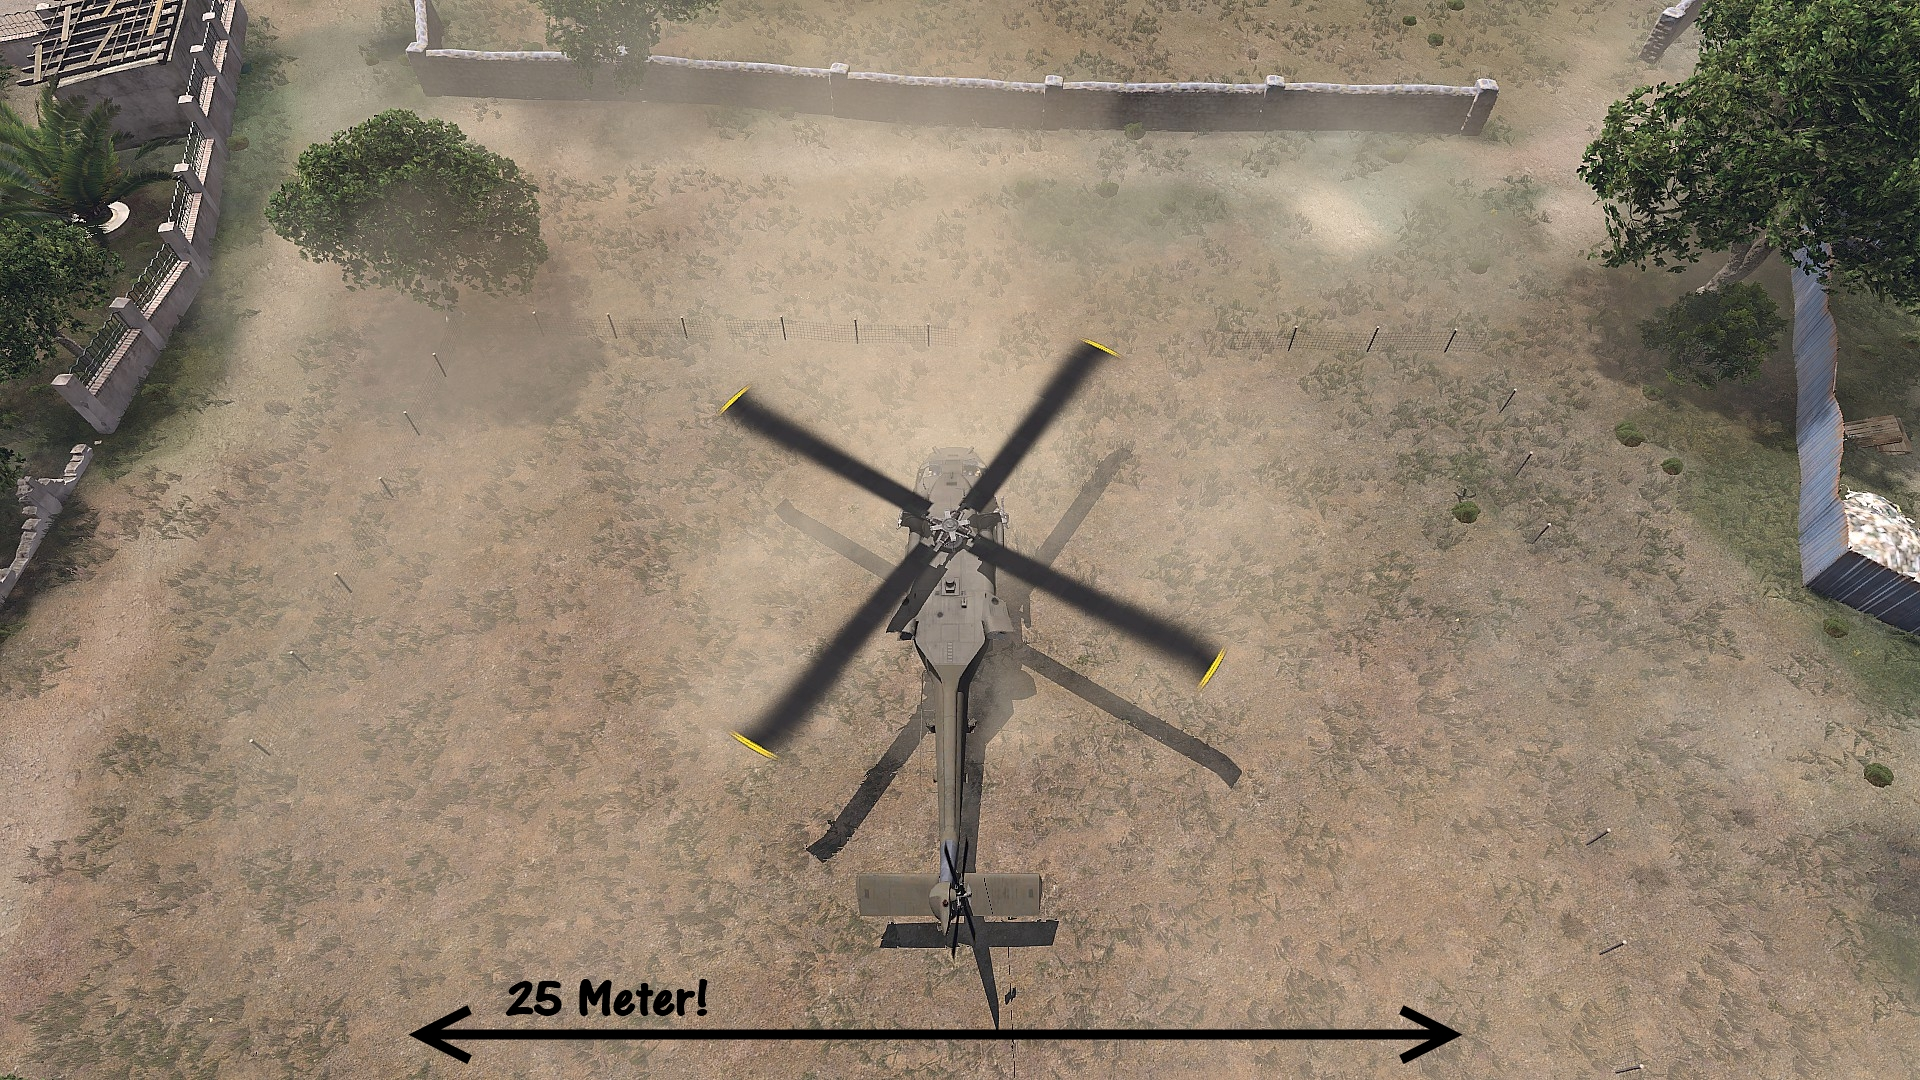
\includegraphics[width=0.95\linewidth]{../img/advanced/hubschrauber_+_infanterie/landezone}
	\end{figure}
	\begin{figure}[htbp]
		\centering
		\includegraphics[width=0.95\linewidth]{../img/advanced/hubschrauber_+_infanterie/verdeckte-landung}
	\end{figure}	

\subsubsection{Heiße Landezonen}
	Bei heißen Landezonen kommt es auf eine gute Reaktion der Infanterie und vor allem Schnelligkeit an. Zur besseren Deckung können die Soldaten Rauchgranaten einsetzen, ebenso kann der Pilot das Einrauchen der Landezone befehlen, um die Sichtlinie zu eventuellen Feindkräften zu brechen.\par
	Wenn ein Helikopter eine bereits unter Beschuss stehende Landezone anfliegen soll, ist der Pilot im Voraus darüber zu unterrichten. Da der Pilot zu jedem Zeitpunkt die vollständige Verantwortung über das Luftfahrzeug inkl. Besatzung inne hat, kann dieser zu jedem Zeitpunkt den Anflug abbrechen oder die Landezone verlassen.\par
	Eine Besonderheit stellt das Aufsitzen der Infanterie unter Beschuss dar hierbei wird die normale Aufsitzreihenfolge missachtet, um ein schnelles Aufsitzen der gesamten Kräfte zu ermöglichen.

\subsection{Informationsfluss}
	Die Helikopterbesatzung wird seitens der OPL über die Anforderung der Ressource mit Angabe des Antragstellers informiert. Nach Bestätigung des Auftrags verbindet sich die Besatzung direkt mit dem jeweiligen Trupp und meldet Einsatzbereitschaft. Nun muss der FAC den im Voraus vorbereiteten 5-Liner an die Besatzung übermitteln. Nach erfolgreichem Readback setzt sich der Helikopter in Bewegung und hält ständigen Funkkontakt, um ggf. plötzliche Änderungen oder wichtige Hinweise durchzugeben oder seitens des FACs zu erhalten.
	\par\medskip
	In Sonderfällen kann der FAC die Ressource zunächst in eine Holding Postition beauftragen und im Anschluss, je nach Situationslage, den 5-Liner an die Besatzung übermitteln oder den Einsatz komplett abbrechen.
	\par\medskip 
	Anmerkung: Falls die Verbindung zwischen Helikopter und FAC ausfallen sollte, wählt sich der Pilot selbstständig sofort auf dem SR Kanal des Trupps ein, um eine Funkverbindung wiederherzustellen.

\subsection{Landeanflug - Die Einweisung/ die Übergabe an den Einweiser}
	Der Pilot meldet die Annäherung an den Operationsraum. In diesem Moment geht die komplette Verantwortung zum FAC über. Er befiehlt dem FAC das markieren der Landezone durch Leucht oder Rauchmarkierungen. Der FAC weist auf Anforderung den Piloten in die korrekte Position ein und warnt ihn ggf. über Gefahren.\par
	Tipp: Bei Nacht sieht man sehr gut ein Knicklicht in Kombination mit einer Rauchgranate, welche darauf geschmissen wird.
	\par\medskip
	Sobald der Pilot den “Touchdown” durchgibt darf die Infanterie die nötigen Aufgaben durchführen.\par
	Warum man einen FAC braucht, hier in einem Video verdeutlicht:\\
	\url{https://www.youtube.com/watch?v=NJIZTL2ZyEw}

	\begin{figure}[htbp]
		\centering
		\includegraphics[width=0.95\linewidth]{../img/advanced/hubschrauber_+_infanterie/sicht-pilot}
	\end{figure}

\subsection{Lift-off}
	Sobald alle Aufgaben abgeschlossen sind oder der FAC die vollständige Anwesenheit durchgibt, führt der Pilot den Lift-off durch. In diesem Moment erlischt die Verantwortung vom FAC. 

\subsection{Worst Case Szenarios}
	Falls während dem Flug die Maschine beschädigt wird, werden alle Pläne und Aufträge verworfen. In diesem Moment ist oberste Priorität die Maschine unversehrt zu landen. In dem Fall, dass ein Helikopter bei einer Landung beschädigt wird, sind die nötigen Maßnahmen zu veranlassen den Helikopter wieder Instand zu setzen.
\pagebreak
\chapter{Fallschirmjäger}

\subsection{Fahrzeuge}
\begin{longtable}{lcccc} 
	\toprule
	Typ & C-130 & CH-47 &	Huron	&	Mohawk \\ 
	\midrule
	Passagiere 	&	25 	&	25 	&	18 	&	16 \\ 
	Min. Sprunghöhe	& 500\,m 	& 300\,m 	&	300\,m	&	300\,m	\\
	Max. Sprunghöhe	&	1000\,m 	&	500\,m 	&	500\,m	&	500\,m \\
	Min. Geschwindigkeit	& 	200\,km/h	&	120\,km/h	&	120\,km/h	&	120\,km/h	\\ 
	Max. Geschwindigkeit	& 	250\,km/h	&	150\,km/h &	150\,km/h &	150\,km/h \\
	\bottomrule 
\end{longtable}

\subsection{Sprungvorbereitung}
\subsubsection*{Kartenvorbereitung}
\begin{tabular}{C{0.1\linewidth}m{0.2\linewidth} m{0.65\linewidth}}
	\includegraphics[scale=0.8]{../img/advanced/fallschirmspringen/sammelzone}	& Sammelzone (SZ)	& ist der Punkt wo sich ein Trupp sammelt, es werden immer 2 Sammelzonen pro Trupp bestimmt\\
	\includegraphics[scale=0.8]{../img/advanced/fallschirmspringen/wendepunkt} 	& Wendepunkt (WP) & Pilot übergibt Loadmaster Befehlsgewalt, letzte Vorbereitung vor Sprung\\
	\includegraphics[scale=0.8]{../img/advanced/fallschirmspringen/dropzone}	& Dropzone (DZ) & ab hier beginnt der Loadmaster mit dem Sprung
\end{tabular}

\subsubsection*{Materialvorbereitung\,/\,Aufsitzen}
\begin{enumerate}
	\item Rucksack auf den Bauch schnallen 
	\item Fallschirm sowie Höhenmesser aus der speziellen Kiste entnehmen
	\item im Trupp vor der Maschine aufstellen; der Loadmaster ist der letzte der einsteigt
	\item im Fahrzeug den Höhenmesser aktivieren \keys{O}\ \underline{selbstständig} und \underline{ohne} Funkbestätigung auf die SR 200 (Sprungfrequenz) wechseln
	\item Truppführer meldet aufsitzen auf der SR 200
\end{enumerate}

\begin{flushright}
	Merke: >>Der Erste wird der Letzte sein.<< 
\end{flushright} 


\subsection{Loadmaster}
Der Loadmaster hat die primäre Aufgabe den Absprung in der Luft zu koordinieren, darunter fällt
zum Beispiel welcher Trupp springt zu welcher Zeit. Des weiteren wird nur auf sein Kommando
gesprungen.

\subsubsection*{Teil der Truppe}
	Die Rolle des Loadmasters wird von ein Mitglied des zuletzt springenden Trupps wahrgenommen.
	Der Loadmaster springt immer als letztes ab, egal welche Position er im Trupp hat.

\subsubsection*{Teil des Fahrzeugteams}
	Die Rolle des Loadmaster wird von einem dritten Mann im Fahrzeug wahrgenommen. Dieser springt am Ende nicht ab, sondern verbleibt im Fahrzeug.

\subsection{Der Sprung}
\subsubsection*{Verhalten beim Sprung}
	Der Fallschirm wird sofort nach Verlassen des Fahrzeuges geöffnet.
	
\subsubsection*{Besonderheiten von ACE3}
	Durch die Modifikation ACE3 kann es vorkommen, dass sich der Fallschirm nicht öffnet. Sollte dies der Fall sein, so muss man durch das ACE-Eigenmenü \keys{StrG+Win} den Fallschirm abschneiden. Anschließend kann man einen Reservefallschirm öffnen, dieser ist jedoch nicht steuerbar.

\subsection{Der Flug}
	Während des gesamten Fluges sollte man versuchen die maximal Geschwindigkeit von 9m/s zu halten, außerdem ist es hilfreich sich beim Navigieren an seinem Vordermann zu orientieren.

\subsection{Die Landung}
\begin{enumerate}
	\item beginnt ab einer Höhe von 50\,m; von da an beträgt die maximal Geschwindigkeit 5m/s,
	\item 20m vor der Landung auf mindestens 3\,m/s abbremsen,
	\item sollte mit maximal 2\,m/s oder weniger erfolgen um Verletzungen zu vermeiden.
\end{enumerate}

\subsection{Sammeln}
\begin{enumerate}
	\item Nach der Landung wird über den Truppfunk das erfolgreiche Landen gemeldet.
	\item Es wird sich eigenständig zur ersten Sammelzone begeben (dafür sind 5min vorgesehen).
	\item Wenn der Trupp vollständig an der ersten Sammelzone ist, bewegt sich dieser zur zweiten
	Sammelzone. Sollten es nicht alle Kameraden zur ersten Sammelzone schaffen bzw. sich
	nach der Landung nicht melden, wird die Suche nach den vermissten Kameraden
	aufgenommen.
	\item Beim Erreichen des zweiten Brückenkopfes ist der Fallschirmsprung abgeschlossen.
\end{enumerate}	
%\chapter{Truppenordnung}
In diesem Abschnitt werden die einzelnen Strukturelemente und die Organisation des \ac{TTT} während einer typischen Mission erklärt.\\
Die hier vorgestellten Strukturen basieren dabei auf der im Laufe der Zeit gesammelten Erfahrung, was in ArmA funktioniert und was nicht und sind verpflichtende Vorgabe für jeden Missionsbauer. Ausnahmen von diesen Strukturen müssen vorher angefragt und genehmigt werden.\\
Da im \ac{TTT} sowohl deutsche als auch amerikanische Strukturen benutzt werden, werden die amerikanischen Namen jeweils in Klammern zusätzlich zu den deutschen Namen genannt.

\section{\acf{OPL} / \acf{HQ}}
\begin{wrapfigure}{r}{0.35\textwidth}
	%\vspace{-15pt}
	\centering 
	\includegraphics[width=0.3\textwidth]{../img/truppenordnung/opl/opl}
	%\caption{Beispiel einer \ac{OPL}}
	%\vspace{-30pt}
\end{wrapfigure}	

Die \ac{OPL} ist die höchste Instanz innerhalb einer Mission. Sie hat den Oberbefehl über alle Einheiten inne, koordiniert das allgemeine Vorgehen innerhalb der Mission und verwaltet die Zuordnung der unterstützenden Einheiten zu den kämpfenden Einheiten. Sie kommuniziert grundsätzlich nur über die Long-Range mit ihren untergeordneten Einheiten.
\par\bigskip
Die \ac{OPL} ist folgendermaßen aufgebaut:
\begin{itemize}
	\item Operationsleiter\,/\,\acs{OPL} (\acf{CO}): Der Oberbefehlshaber der Mission. Er gibt die Befehle und erstellt "den großen Plan".
	\item stellv. \ac{OPL} (\acf{XO}): Unterstützt den \ac{OPL} bei seinen Aufgaben, typischerweise beim Funken mit den untergeordneten Trupps. Kann jedoch auch alle weiteren Aufgaben übernehmen, die ihm der \ac{OPL} überträgt -- er ist Mädchen für alles. Bewährt hat sich das Prinzip, dass der \ac{OPL} den eingehenden Funk übernimmt (Anfragen von anderen Trupps) und der stellv. \ac{OPL} den ausgehenden Funk (Abfragen von Statusberichten, Übermittlung von neuen Befehlen).
\end{itemize}
Ergänzt werden kann die \ac{OPL} durch maximal 4 Spieler, welche folgende Rollen einnehmen können:
\begin{itemize}
	\item Funker (\acf{RO}): ein zusätzlicher Funker, um die \ac{OPL} zu unterstützen, kann auf eine Spezialrolle beschränkt sein und für diese eine eigene LR-Frequenz bekommen (so kann es z.\,B. bei einer Mission mit vielen Lufteinheiten sinnvoll sein, jemanden zu haben, der sich auf einer eigenen Frequenz nur um die Koordination der Lufteinheiten um das Flugfeld kümmert und zentraler Ansprechpartner aller Lufteinheiten für Start-\,/\,Landemanöver ist)
	\item Aufklärungsoffizier (\acf{IO}): Sammelt alle verfügbaren, relevanten Daten und leitet diese gegebenenfalls an andere Trupps weiter. Hat meistens eine eigene, "große" Drohne (Greyhawk\,/\,Global Hawk) zur Feindaufklärung.
	\item freie Rolle (maximal einmal): je nach Mission kann es sinnvoll sein, dem \ac{OPL} einen Sanitäter, einen Nahsicherer, einen Fahrer o.\,Ä. zur Seite zu stellen
\end{itemize}
Je nach Größe und Struktur der Mission kann die \ac{OPL} identisch sein mit
\begin{itemize}
	\item der Sektionsführung, falls die Truppstruktur der Mission nur aus einer Sektion besteht
	\item der Zugführung, falls die Truppstruktur der Mission nur aus einem Zug besteht (egal ob Infanteriezug, Panzerzug oder mechanisierte Infanterie). Dies ist die einzige Ausnahme, in der die \ac{OPL} per Short-Range statt Long-Range mit ihren untergeordneten Einheiten kommuniziert.
\end{itemize}
Die OPL hält typischerweise einen sehr großen Abstand zu ihren Truppen - oft bleibt sie auch durchgehend in der Basis.

\section{Sektionsführung / Platoon Lead (PLT)}
\begin{wrapfigure}{r}{0.4\textwidth}
	\vspace{-25pt}
	\centering 
	\includegraphics[width=0.3\textwidth]{./img/truppenordnung/sektionsfuehrung/sektionsfuehrung}
	%\caption{Beispiel einer Sektionsführung}
	\vspace{-90pt}
\end{wrapfigure}	
Die Sektionsführung ist ein Bindeglied zwischen OPL und Zugführung, um die OPL zu entlasten. Einer Sektionsführung sind mindestens zwei, maximal vier Züge unterstellt. Ab drei Zügen in einer Mission ist die Sektionsführung zwingend erforderlich, darunter optional.\\

Die Sektionsführung ist folgendermaßen aufgebaut:
\begin{itemize}
	\item Sektionsführer\,/\,Platoon Lead (PLT): Er leitet die ihm untergeordneten Züge. Kommuniziert wird über Long-Range - entweder über die individuellen Frequenzen der einzelnen Züge oder über die Task-Force-Frequenz (siehe nächstes Kapitel).
	\item Funker / Radio Operator (RO): Übernimmt die Kommunikation zur OPL und anderen Einheiten.
\end{itemize}
Ergänzt werden kann die Sektionsführung bei Bedarf durch:
\begin{itemize}
	\setlength\itemsep{0em}
	\item einen Gefechtssanitäter\,/\,Combat Medic (CM) zur Versorgung im Feld.
	\item einen Fahrzeugführer\,/\,Nahsicherer zur selbstständigen Verlegung
\end{itemize} 
Die Sektionsführung befindet sich typischerweise etwas weiter entfernt hinter den ihr unterstellten Zügen.

\input{./tex/truppenordnung/zugfuehrung/zugfuehrung}
\section{Infanterietrupp / Fireteam (FT)}
\begin{wrapfigure}{R}{0.35\textwidth}
	\vspace{-50pt}
	\centering 
	\includegraphics[width=0.2\textwidth]{../img/truppenordnung/infanterie/infanterie}
	%\caption{Beispiel eines Infantrietrupps}
	\vspace{-90pt}
\end{wrapfigure}
Die Infanterie bildet den Kernbestandteil vieler Missionen. Ein Infanterietrupp ist immer Teil eines Zuges und besteht aus 4 oder 6 Mann. Mögliche Positionen innerhalb eines Infanterietrupps sind:
\vspace{3.5cm}
\begin{longtable}{@{}P{0.4\textwidth}P{0.4\textwidth}@{}}
	\toprule
	Deutsche Bezeichnung & Englische Bezeichnung\\
	\midrule
	Truppführer (TF) & Fireteam Leader (FTL)\\
	Grenadier (GRE) & \\
	Leichter MG-Schütze (LMG) & Automatic Rifleman (AR)\\
	Mittlerer MG-Schütze & Medium Machine Gunner (MMG) \\
	MG-Assistent & Assistant Machine Gunner (AMG)\footnote{notwendig für MMG}\\ 
	Leichter Panzerabwehrschütze & Light Anti Tank (LAT)\\
	Schwerer Panzerabwehrschütze & Heavy Anti Tank (HAT)\\
	Panzerabwehr-Assistent & Assistant Anti Tank (AAT)\footnote{notwendig für HAT}\\ 
	Luftabwehrschütze & Anti-Air (AA)\\
	Pionier & Pioneer (PIO)\\
	Gefechtssanitäter & Combat Medic (CM)\\
	Schütze & Rifleman (RI)\\			
	\bottomrule					
\end{longtable}


Auf eine sinnvolle Einteilung in Buddy"=Teams (z.\,B. bei Positionen, die einen Assistenten erfordern), ist hierbei zu achten.\\
Die Kommunikation erfolgt ausschließlich über Short-Range, der Truppführer schaltet sich über seine Additional-Short-Range auf den Zugkanal auf, um sich mit der Zugführung und den anderen Truppführern im Zug abzusprechen. Die Nummer 2 im Trupp kann sich ebenfalls auf den Zugfunk aufschalten, jedoch nur mithören und nicht funken -- es sei denn, der Truppführer fällt aus und die Nummer 2 übernimmt.

\section{Spezialtrupp}
\includegraphics[width=20mm]{./img/truppenordnung/spezialeinheiten/sf1}\quad
\includegraphics[width=20mm]{./img/truppenordnung/spezialeinheiten/sf2}\\
Spezialtruppen sind infanteristische Einheiten bestehend aus zwei bis sechs Mann mit einem klaren Aufgabenschwerpunkt -- dies kann vom klassischen Zwei"=Mann"=Scharfschützenteam bis zum Sechs-Mann-Kampftauchertrupp gehen. Sie sind die flexibelsten Einheiten innerhalb des TTTs und können entweder autark arbeiten oder im Verbund mit einem anderen Trupp oder Zug. Pro Mission existieren maximal zwei autark operierende Spezialtruppen, im Verbund mit einem Zug maximal einer.\\
Kommunikation erfolgt über Long"=Range, beim Arbeiten im Verbund zusätzlich über die Additional"=Short"=Range (Zugfunk). Kämpfende Einheiten wie z.B. Kommandotrupps oder Kampftaucher, in denen der Truppführer viel Mikromanagement leisten und der Trupp in direkte Feuergefechte verwickelt wird, benötigen zwingend einen separaten Funker. In unterstützenden Einheiten wie z.B. Aufklärungsteams oder Mörserteams, die voraussichtlich nicht in direkte Feuergefechte verwickelt werden, kann (muss aber nicht) der Truppführer die Long"=Range"=Kommunikation mit übernehmen.\\
Mögliche Aufgabenschwerpunkte eines Spezialtrupps sind z.B.:

\begin{itemize}
	\setlength\itemsep{0em}
	\item JTAC-Team
	\item Aufklärungsteam (UAV)
	\item Autonome Kampfeinheit (UGV)
	\item Mörserteam
	\item schwere Feuerunterstützung (Schweres Maschinengewehr (HMG) / Granatmaschinengewehr (GMG))
	\item (schwere) Panzerabwehr / Flugabwehr (falls nicht bereits im Zug vorhanden)
	\item Pionier-Team (falls nicht bereits im Zug vorhanden)
	\item medizinische Versorgung/Unterstützung (falls kein MedEvac in der Mission vorhanden)
	\item Kommandokräfte (Infiltration)
	\item Scharfschützenteam
	\item Kampftaucher
\end{itemize}
Bei entsprechenden Rollen (schwere Waffen, Mörser, etc.) ist auf das Vorhandensein eines entsprechenden Assistenten zu achten.
\section{Logistik}
\includegraphics[width=20mm]{../img/truppenordnung/logistikMedevac/silber}\linebreak
Silber -- Bussard -- Stellt Fahrzeuge und Personal bereit, mit denen Transport und Logistik durchgeführt werden.
\section{MedEvac}
\includegraphics[width=20mm]{../img/truppenordnung/logistikMedevac/weiss}\\
Weiß -- \acf{MedEvac} -- Unterstützt Operationen mit Versorgungs- und Transportkapazität für Verwundete.
\section{Close Air Support}
\includegraphics[width=20mm]{../img/truppenordnung/logistikMedevac/silber}\\
Silber -- Adler -- Stellt Fahrzeuge und Personal bereit,  Gefechtsunterstützung (\ac{CAS}) und Geleitschutz durchgeführt werden.
\input{./tex/truppenordnung/mechanisierteInfanterie/mechanisierte_infanterie}
\input{./tex/truppenordnung/kampfpanzer/kampfpanzer}
\input{./tex/truppenordnung/artillerie/artillerie}
\chapter{Truppenordnung}
In diesem Abschnitt werden die einzelnen Strukturelemente und die Organisation des \ac{TTT} während einer typischen Mission erklärt.\\
Die hier vorgestellten Strukturen basieren dabei auf der im Laufe der Zeit gesammelten Erfahrung, was in ArmA funktioniert und was nicht und sind verpflichtende Vorgabe für jeden Missionsbauer. Ausnahmen von diesen Strukturen müssen vorher angefragt und genehmigt werden.\\
Da im \ac{TTT} sowohl deutsche als auch amerikanische Strukturen benutzt werden, werden die amerikanischen Namen jeweils in Klammern zusätzlich zu den deutschen Namen genannt.

\section{\acf{OPL} / \acf{HQ}}
\begin{wrapfigure}{r}{0.35\textwidth}
	%\vspace{-15pt}
	\centering 
	\includegraphics[width=0.3\textwidth]{../img/truppenordnung/opl/opl}
	%\caption{Beispiel einer \ac{OPL}}
	%\vspace{-30pt}
\end{wrapfigure}	

Die \ac{OPL} ist die höchste Instanz innerhalb einer Mission. Sie hat den Oberbefehl über alle Einheiten inne, koordiniert das allgemeine Vorgehen innerhalb der Mission und verwaltet die Zuordnung der unterstützenden Einheiten zu den kämpfenden Einheiten. Sie kommuniziert grundsätzlich nur über die Long-Range mit ihren untergeordneten Einheiten.
\par\bigskip
Die \ac{OPL} ist folgendermaßen aufgebaut:
\begin{itemize}
	\item Operationsleiter\,/\,\acs{OPL} (\acf{CO}): Der Oberbefehlshaber der Mission. Er gibt die Befehle und erstellt "den großen Plan".
	\item stellv. \ac{OPL} (\acf{XO}): Unterstützt den \ac{OPL} bei seinen Aufgaben, typischerweise beim Funken mit den untergeordneten Trupps. Kann jedoch auch alle weiteren Aufgaben übernehmen, die ihm der \ac{OPL} überträgt -- er ist Mädchen für alles. Bewährt hat sich das Prinzip, dass der \ac{OPL} den eingehenden Funk übernimmt (Anfragen von anderen Trupps) und der stellv. \ac{OPL} den ausgehenden Funk (Abfragen von Statusberichten, Übermittlung von neuen Befehlen).
\end{itemize}
Ergänzt werden kann die \ac{OPL} durch maximal 4 Spieler, welche folgende Rollen einnehmen können:
\begin{itemize}
	\item Funker (\acf{RO}): ein zusätzlicher Funker, um die \ac{OPL} zu unterstützen, kann auf eine Spezialrolle beschränkt sein und für diese eine eigene LR-Frequenz bekommen (so kann es z.\,B. bei einer Mission mit vielen Lufteinheiten sinnvoll sein, jemanden zu haben, der sich auf einer eigenen Frequenz nur um die Koordination der Lufteinheiten um das Flugfeld kümmert und zentraler Ansprechpartner aller Lufteinheiten für Start-\,/\,Landemanöver ist)
	\item Aufklärungsoffizier (\acf{IO}): Sammelt alle verfügbaren, relevanten Daten und leitet diese gegebenenfalls an andere Trupps weiter. Hat meistens eine eigene, "große" Drohne (Greyhawk\,/\,Global Hawk) zur Feindaufklärung.
	\item freie Rolle (maximal einmal): je nach Mission kann es sinnvoll sein, dem \ac{OPL} einen Sanitäter, einen Nahsicherer, einen Fahrer o.\,Ä. zur Seite zu stellen
\end{itemize}
Je nach Größe und Struktur der Mission kann die \ac{OPL} identisch sein mit
\begin{itemize}
	\item der Sektionsführung, falls die Truppstruktur der Mission nur aus einer Sektion besteht
	\item der Zugführung, falls die Truppstruktur der Mission nur aus einem Zug besteht (egal ob Infanteriezug, Panzerzug oder mechanisierte Infanterie). Dies ist die einzige Ausnahme, in der die \ac{OPL} per Short-Range statt Long-Range mit ihren untergeordneten Einheiten kommuniziert.
\end{itemize}
Die OPL hält typischerweise einen sehr großen Abstand zu ihren Truppen - oft bleibt sie auch durchgehend in der Basis.

\section{Sektionsführung / Platoon Lead (PLT)}
\begin{wrapfigure}{r}{0.4\textwidth}
	\vspace{-25pt}
	\centering 
	\includegraphics[width=0.3\textwidth]{./img/truppenordnung/sektionsfuehrung/sektionsfuehrung}
	%\caption{Beispiel einer Sektionsführung}
	\vspace{-90pt}
\end{wrapfigure}	
Die Sektionsführung ist ein Bindeglied zwischen OPL und Zugführung, um die OPL zu entlasten. Einer Sektionsführung sind mindestens zwei, maximal vier Züge unterstellt. Ab drei Zügen in einer Mission ist die Sektionsführung zwingend erforderlich, darunter optional.\\

Die Sektionsführung ist folgendermaßen aufgebaut:
\begin{itemize}
	\item Sektionsführer\,/\,Platoon Lead (PLT): Er leitet die ihm untergeordneten Züge. Kommuniziert wird über Long-Range - entweder über die individuellen Frequenzen der einzelnen Züge oder über die Task-Force-Frequenz (siehe nächstes Kapitel).
	\item Funker / Radio Operator (RO): Übernimmt die Kommunikation zur OPL und anderen Einheiten.
\end{itemize}
Ergänzt werden kann die Sektionsführung bei Bedarf durch:
\begin{itemize}
	\setlength\itemsep{0em}
	\item einen Gefechtssanitäter\,/\,Combat Medic (CM) zur Versorgung im Feld.
	\item einen Fahrzeugführer\,/\,Nahsicherer zur selbstständigen Verlegung
\end{itemize} 
Die Sektionsführung befindet sich typischerweise etwas weiter entfernt hinter den ihr unterstellten Zügen.

\input{./tex/truppenordnung/zugfuehrung/zugfuehrung}
\section{Infanterietrupp / Fireteam (FT)}
\begin{wrapfigure}{R}{0.35\textwidth}
	\vspace{-50pt}
	\centering 
	\includegraphics[width=0.2\textwidth]{../img/truppenordnung/infanterie/infanterie}
	%\caption{Beispiel eines Infantrietrupps}
	\vspace{-90pt}
\end{wrapfigure}
Die Infanterie bildet den Kernbestandteil vieler Missionen. Ein Infanterietrupp ist immer Teil eines Zuges und besteht aus 4 oder 6 Mann. Mögliche Positionen innerhalb eines Infanterietrupps sind:
\vspace{3.5cm}
\begin{longtable}{@{}P{0.4\textwidth}P{0.4\textwidth}@{}}
	\toprule
	Deutsche Bezeichnung & Englische Bezeichnung\\
	\midrule
	Truppführer (TF) & Fireteam Leader (FTL)\\
	Grenadier (GRE) & \\
	Leichter MG-Schütze (LMG) & Automatic Rifleman (AR)\\
	Mittlerer MG-Schütze & Medium Machine Gunner (MMG) \\
	MG-Assistent & Assistant Machine Gunner (AMG)\footnote{notwendig für MMG}\\ 
	Leichter Panzerabwehrschütze & Light Anti Tank (LAT)\\
	Schwerer Panzerabwehrschütze & Heavy Anti Tank (HAT)\\
	Panzerabwehr-Assistent & Assistant Anti Tank (AAT)\footnote{notwendig für HAT}\\ 
	Luftabwehrschütze & Anti-Air (AA)\\
	Pionier & Pioneer (PIO)\\
	Gefechtssanitäter & Combat Medic (CM)\\
	Schütze & Rifleman (RI)\\			
	\bottomrule					
\end{longtable}


Auf eine sinnvolle Einteilung in Buddy"=Teams (z.\,B. bei Positionen, die einen Assistenten erfordern), ist hierbei zu achten.\\
Die Kommunikation erfolgt ausschließlich über Short-Range, der Truppführer schaltet sich über seine Additional-Short-Range auf den Zugkanal auf, um sich mit der Zugführung und den anderen Truppführern im Zug abzusprechen. Die Nummer 2 im Trupp kann sich ebenfalls auf den Zugfunk aufschalten, jedoch nur mithören und nicht funken -- es sei denn, der Truppführer fällt aus und die Nummer 2 übernimmt.

\section{Spezialtrupp}
\includegraphics[width=20mm]{./img/truppenordnung/spezialeinheiten/sf1}\quad
\includegraphics[width=20mm]{./img/truppenordnung/spezialeinheiten/sf2}\\
Spezialtruppen sind infanteristische Einheiten bestehend aus zwei bis sechs Mann mit einem klaren Aufgabenschwerpunkt -- dies kann vom klassischen Zwei"=Mann"=Scharfschützenteam bis zum Sechs-Mann-Kampftauchertrupp gehen. Sie sind die flexibelsten Einheiten innerhalb des TTTs und können entweder autark arbeiten oder im Verbund mit einem anderen Trupp oder Zug. Pro Mission existieren maximal zwei autark operierende Spezialtruppen, im Verbund mit einem Zug maximal einer.\\
Kommunikation erfolgt über Long"=Range, beim Arbeiten im Verbund zusätzlich über die Additional"=Short"=Range (Zugfunk). Kämpfende Einheiten wie z.B. Kommandotrupps oder Kampftaucher, in denen der Truppführer viel Mikromanagement leisten und der Trupp in direkte Feuergefechte verwickelt wird, benötigen zwingend einen separaten Funker. In unterstützenden Einheiten wie z.B. Aufklärungsteams oder Mörserteams, die voraussichtlich nicht in direkte Feuergefechte verwickelt werden, kann (muss aber nicht) der Truppführer die Long"=Range"=Kommunikation mit übernehmen.\\
Mögliche Aufgabenschwerpunkte eines Spezialtrupps sind z.B.:

\begin{itemize}
	\setlength\itemsep{0em}
	\item JTAC-Team
	\item Aufklärungsteam (UAV)
	\item Autonome Kampfeinheit (UGV)
	\item Mörserteam
	\item schwere Feuerunterstützung (Schweres Maschinengewehr (HMG) / Granatmaschinengewehr (GMG))
	\item (schwere) Panzerabwehr / Flugabwehr (falls nicht bereits im Zug vorhanden)
	\item Pionier-Team (falls nicht bereits im Zug vorhanden)
	\item medizinische Versorgung/Unterstützung (falls kein MedEvac in der Mission vorhanden)
	\item Kommandokräfte (Infiltration)
	\item Scharfschützenteam
	\item Kampftaucher
\end{itemize}
Bei entsprechenden Rollen (schwere Waffen, Mörser, etc.) ist auf das Vorhandensein eines entsprechenden Assistenten zu achten.
\section{Logistik}
\includegraphics[width=20mm]{../img/truppenordnung/logistikMedevac/silber}\linebreak
Silber -- Bussard -- Stellt Fahrzeuge und Personal bereit, mit denen Transport und Logistik durchgeführt werden.
\section{MedEvac}
\includegraphics[width=20mm]{../img/truppenordnung/logistikMedevac/weiss}\\
Weiß -- \acf{MedEvac} -- Unterstützt Operationen mit Versorgungs- und Transportkapazität für Verwundete.
\section{Close Air Support}
\includegraphics[width=20mm]{../img/truppenordnung/logistikMedevac/silber}\\
Silber -- Adler -- Stellt Fahrzeuge und Personal bereit,  Gefechtsunterstützung (\ac{CAS}) und Geleitschutz durchgeführt werden.
\input{./tex/truppenordnung/mechanisierteInfanterie/mechanisierte_infanterie}
\input{./tex/truppenordnung/kampfpanzer/kampfpanzer}
\input{./tex/truppenordnung/artillerie/artillerie}
%\chapter{Truppenordnung}
In diesem Abschnitt werden die einzelnen Strukturelemente und die Organisation des \ac{TTT} während einer typischen Mission erklärt.\\
Die hier vorgestellten Strukturen basieren dabei auf der im Laufe der Zeit gesammelten Erfahrung, was in ArmA funktioniert und was nicht und sind verpflichtende Vorgabe für jeden Missionsbauer. Ausnahmen von diesen Strukturen müssen vorher angefragt und genehmigt werden.\\
Da im \ac{TTT} sowohl deutsche als auch amerikanische Strukturen benutzt werden, werden die amerikanischen Namen jeweils in Klammern zusätzlich zu den deutschen Namen genannt.

\section{\acf{OPL} / \acf{HQ}}
\begin{wrapfigure}{r}{0.35\textwidth}
	%\vspace{-15pt}
	\centering 
	\includegraphics[width=0.3\textwidth]{../img/truppenordnung/opl/opl}
	%\caption{Beispiel einer \ac{OPL}}
	%\vspace{-30pt}
\end{wrapfigure}	

Die \ac{OPL} ist die höchste Instanz innerhalb einer Mission. Sie hat den Oberbefehl über alle Einheiten inne, koordiniert das allgemeine Vorgehen innerhalb der Mission und verwaltet die Zuordnung der unterstützenden Einheiten zu den kämpfenden Einheiten. Sie kommuniziert grundsätzlich nur über die Long-Range mit ihren untergeordneten Einheiten.
\par\bigskip
Die \ac{OPL} ist folgendermaßen aufgebaut:
\begin{itemize}
	\item Operationsleiter\,/\,\acs{OPL} (\acf{CO}): Der Oberbefehlshaber der Mission. Er gibt die Befehle und erstellt "den großen Plan".
	\item stellv. \ac{OPL} (\acf{XO}): Unterstützt den \ac{OPL} bei seinen Aufgaben, typischerweise beim Funken mit den untergeordneten Trupps. Kann jedoch auch alle weiteren Aufgaben übernehmen, die ihm der \ac{OPL} überträgt -- er ist Mädchen für alles. Bewährt hat sich das Prinzip, dass der \ac{OPL} den eingehenden Funk übernimmt (Anfragen von anderen Trupps) und der stellv. \ac{OPL} den ausgehenden Funk (Abfragen von Statusberichten, Übermittlung von neuen Befehlen).
\end{itemize}
Ergänzt werden kann die \ac{OPL} durch maximal 4 Spieler, welche folgende Rollen einnehmen können:
\begin{itemize}
	\item Funker (\acf{RO}): ein zusätzlicher Funker, um die \ac{OPL} zu unterstützen, kann auf eine Spezialrolle beschränkt sein und für diese eine eigene LR-Frequenz bekommen (so kann es z.\,B. bei einer Mission mit vielen Lufteinheiten sinnvoll sein, jemanden zu haben, der sich auf einer eigenen Frequenz nur um die Koordination der Lufteinheiten um das Flugfeld kümmert und zentraler Ansprechpartner aller Lufteinheiten für Start-\,/\,Landemanöver ist)
	\item Aufklärungsoffizier (\acf{IO}): Sammelt alle verfügbaren, relevanten Daten und leitet diese gegebenenfalls an andere Trupps weiter. Hat meistens eine eigene, "große" Drohne (Greyhawk\,/\,Global Hawk) zur Feindaufklärung.
	\item freie Rolle (maximal einmal): je nach Mission kann es sinnvoll sein, dem \ac{OPL} einen Sanitäter, einen Nahsicherer, einen Fahrer o.\,Ä. zur Seite zu stellen
\end{itemize}
Je nach Größe und Struktur der Mission kann die \ac{OPL} identisch sein mit
\begin{itemize}
	\item der Sektionsführung, falls die Truppstruktur der Mission nur aus einer Sektion besteht
	\item der Zugführung, falls die Truppstruktur der Mission nur aus einem Zug besteht (egal ob Infanteriezug, Panzerzug oder mechanisierte Infanterie). Dies ist die einzige Ausnahme, in der die \ac{OPL} per Short-Range statt Long-Range mit ihren untergeordneten Einheiten kommuniziert.
\end{itemize}
Die OPL hält typischerweise einen sehr großen Abstand zu ihren Truppen - oft bleibt sie auch durchgehend in der Basis.

\section{Sektionsführung / Platoon Lead (PLT)}
\begin{wrapfigure}{r}{0.4\textwidth}
	\vspace{-25pt}
	\centering 
	\includegraphics[width=0.3\textwidth]{./img/truppenordnung/sektionsfuehrung/sektionsfuehrung}
	%\caption{Beispiel einer Sektionsführung}
	\vspace{-90pt}
\end{wrapfigure}	
Die Sektionsführung ist ein Bindeglied zwischen OPL und Zugführung, um die OPL zu entlasten. Einer Sektionsführung sind mindestens zwei, maximal vier Züge unterstellt. Ab drei Zügen in einer Mission ist die Sektionsführung zwingend erforderlich, darunter optional.\\

Die Sektionsführung ist folgendermaßen aufgebaut:
\begin{itemize}
	\item Sektionsführer\,/\,Platoon Lead (PLT): Er leitet die ihm untergeordneten Züge. Kommuniziert wird über Long-Range - entweder über die individuellen Frequenzen der einzelnen Züge oder über die Task-Force-Frequenz (siehe nächstes Kapitel).
	\item Funker / Radio Operator (RO): Übernimmt die Kommunikation zur OPL und anderen Einheiten.
\end{itemize}
Ergänzt werden kann die Sektionsführung bei Bedarf durch:
\begin{itemize}
	\setlength\itemsep{0em}
	\item einen Gefechtssanitäter\,/\,Combat Medic (CM) zur Versorgung im Feld.
	\item einen Fahrzeugführer\,/\,Nahsicherer zur selbstständigen Verlegung
\end{itemize} 
Die Sektionsführung befindet sich typischerweise etwas weiter entfernt hinter den ihr unterstellten Zügen.

\input{./tex/truppenordnung/zugfuehrung/zugfuehrung}
\section{Infanterietrupp / Fireteam (FT)}
\begin{wrapfigure}{R}{0.35\textwidth}
	\vspace{-50pt}
	\centering 
	\includegraphics[width=0.2\textwidth]{../img/truppenordnung/infanterie/infanterie}
	%\caption{Beispiel eines Infantrietrupps}
	\vspace{-90pt}
\end{wrapfigure}
Die Infanterie bildet den Kernbestandteil vieler Missionen. Ein Infanterietrupp ist immer Teil eines Zuges und besteht aus 4 oder 6 Mann. Mögliche Positionen innerhalb eines Infanterietrupps sind:
\vspace{3.5cm}
\begin{longtable}{@{}P{0.4\textwidth}P{0.4\textwidth}@{}}
	\toprule
	Deutsche Bezeichnung & Englische Bezeichnung\\
	\midrule
	Truppführer (TF) & Fireteam Leader (FTL)\\
	Grenadier (GRE) & \\
	Leichter MG-Schütze (LMG) & Automatic Rifleman (AR)\\
	Mittlerer MG-Schütze & Medium Machine Gunner (MMG) \\
	MG-Assistent & Assistant Machine Gunner (AMG)\footnote{notwendig für MMG}\\ 
	Leichter Panzerabwehrschütze & Light Anti Tank (LAT)\\
	Schwerer Panzerabwehrschütze & Heavy Anti Tank (HAT)\\
	Panzerabwehr-Assistent & Assistant Anti Tank (AAT)\footnote{notwendig für HAT}\\ 
	Luftabwehrschütze & Anti-Air (AA)\\
	Pionier & Pioneer (PIO)\\
	Gefechtssanitäter & Combat Medic (CM)\\
	Schütze & Rifleman (RI)\\			
	\bottomrule					
\end{longtable}


Auf eine sinnvolle Einteilung in Buddy"=Teams (z.\,B. bei Positionen, die einen Assistenten erfordern), ist hierbei zu achten.\\
Die Kommunikation erfolgt ausschließlich über Short-Range, der Truppführer schaltet sich über seine Additional-Short-Range auf den Zugkanal auf, um sich mit der Zugführung und den anderen Truppführern im Zug abzusprechen. Die Nummer 2 im Trupp kann sich ebenfalls auf den Zugfunk aufschalten, jedoch nur mithören und nicht funken -- es sei denn, der Truppführer fällt aus und die Nummer 2 übernimmt.

\section{Spezialtrupp}
\includegraphics[width=20mm]{./img/truppenordnung/spezialeinheiten/sf1}\quad
\includegraphics[width=20mm]{./img/truppenordnung/spezialeinheiten/sf2}\\
Spezialtruppen sind infanteristische Einheiten bestehend aus zwei bis sechs Mann mit einem klaren Aufgabenschwerpunkt -- dies kann vom klassischen Zwei"=Mann"=Scharfschützenteam bis zum Sechs-Mann-Kampftauchertrupp gehen. Sie sind die flexibelsten Einheiten innerhalb des TTTs und können entweder autark arbeiten oder im Verbund mit einem anderen Trupp oder Zug. Pro Mission existieren maximal zwei autark operierende Spezialtruppen, im Verbund mit einem Zug maximal einer.\\
Kommunikation erfolgt über Long"=Range, beim Arbeiten im Verbund zusätzlich über die Additional"=Short"=Range (Zugfunk). Kämpfende Einheiten wie z.B. Kommandotrupps oder Kampftaucher, in denen der Truppführer viel Mikromanagement leisten und der Trupp in direkte Feuergefechte verwickelt wird, benötigen zwingend einen separaten Funker. In unterstützenden Einheiten wie z.B. Aufklärungsteams oder Mörserteams, die voraussichtlich nicht in direkte Feuergefechte verwickelt werden, kann (muss aber nicht) der Truppführer die Long"=Range"=Kommunikation mit übernehmen.\\
Mögliche Aufgabenschwerpunkte eines Spezialtrupps sind z.B.:

\begin{itemize}
	\setlength\itemsep{0em}
	\item JTAC-Team
	\item Aufklärungsteam (UAV)
	\item Autonome Kampfeinheit (UGV)
	\item Mörserteam
	\item schwere Feuerunterstützung (Schweres Maschinengewehr (HMG) / Granatmaschinengewehr (GMG))
	\item (schwere) Panzerabwehr / Flugabwehr (falls nicht bereits im Zug vorhanden)
	\item Pionier-Team (falls nicht bereits im Zug vorhanden)
	\item medizinische Versorgung/Unterstützung (falls kein MedEvac in der Mission vorhanden)
	\item Kommandokräfte (Infiltration)
	\item Scharfschützenteam
	\item Kampftaucher
\end{itemize}
Bei entsprechenden Rollen (schwere Waffen, Mörser, etc.) ist auf das Vorhandensein eines entsprechenden Assistenten zu achten.
\section{Logistik}
\includegraphics[width=20mm]{../img/truppenordnung/logistikMedevac/silber}\linebreak
Silber -- Bussard -- Stellt Fahrzeuge und Personal bereit, mit denen Transport und Logistik durchgeführt werden.
\section{MedEvac}
\includegraphics[width=20mm]{../img/truppenordnung/logistikMedevac/weiss}\\
Weiß -- \acf{MedEvac} -- Unterstützt Operationen mit Versorgungs- und Transportkapazität für Verwundete.
\section{Close Air Support}
\includegraphics[width=20mm]{../img/truppenordnung/logistikMedevac/silber}\\
Silber -- Adler -- Stellt Fahrzeuge und Personal bereit,  Gefechtsunterstützung (\ac{CAS}) und Geleitschutz durchgeführt werden.
\input{./tex/truppenordnung/mechanisierteInfanterie/mechanisierte_infanterie}
\input{./tex/truppenordnung/kampfpanzer/kampfpanzer}
\input{./tex/truppenordnung/artillerie/artillerie}


%Mods
%\part{SGA \& Tutorials}
%\chapter{SGA}
%\input{./special/spz/spz}
%\chapter{Tutorials}
%\input{./special/tfar/tfar}
%\pagebreak

%Sonstiges
%\chapter{Sonstiges}
%%\begin{landscape} %Querformat
\section{nützliche Tastatur (Um)Belegung}
Tipp: Kompass auf >>Leertaste<< legen so ist dieser leichter verfügbar als über die Taste >>K<<
%\end{landscape}
%das Abkürzungsverzeichnis erstellen
\pagebreak
\section*{Abkürzungsverzeichnis}
\addcontentsline{toc}{section}{Abk\"urzungsverzeichnis} 
\begin{acronym}[SEPSEPSEP]
\setlength{\itemsep}{1em}
	\acro{AAR}{After Action Report}
	\acro{OPL}{Operationsleitung}
	\acro{SQL}{Squadlead}
	\acro{FAC}{Forward Air Controler}
	\acro{AT}{Anti Tank}
	\acro{UAV}{Unmanned Aerial Vehicle}
	\acro{TTT}{Tactical Training Team}
	\acro{AA}{Anti Air}
	\acro{KPZ}{Kampfpanzer}	
	\acro{SPZ}{Schützenpanzer}
	\acro{CAS}{Close Air Support}
	\acro{CQB}{Operationsleitung}
	\acro{AGA}{Allgemeine Grundausbildung}
	\acro{SGA}{Spezielle Grundausbildung}
	\acro{KSK}{Kommando Spezialkräfte}
	\acro{MedEvac}{MEDical EVACuation}
	\acro{CSE}{Combat Space Enhancement}
	\acro{IR}{Infrarot}
	\acro{EOD}{Explosive Ordnance Disposal}
	\acro{LZ}{Landezone}
	\acro{KT}{Kampftrupp}
	\acro{SR}{Short Range}
	\acro{LR}{Long Range}
\end{acronym}
\pagebreak

%Ganz zum Schluss
\pagebreak
\chapter*{Autoren}
\addcontentsline{toc}{chapter}{Autoren} 
	Ein herzliches Dank an euch für eure fleißige Mitarbeit, sowie an alle die am \ac{TTT} mitwirken.\\ 
	
	\begin{tabular}{p{0.23\textwidth}p{0.23\textwidth}p{0.23\textwidth}p{0.23\textwidth}}
		Ghost & 
		grauer Wolf &
		Grunt &
		GSG9\_abzocker\\
		Highhead &
		LingLing & 
		Lorddrinkalot &
		Lufros\\
		Mynx &
		Nachti &
		Reimchen &
		Relain\\
		Schotte &
		SCiite &
		Speutzi &
		Stura \\
		TheConen\\
	\end{tabular}	

\cleardoublepage
\appendix
\end{document}